\documentclass{article}

\usepackage[italian]{babel} 
\usepackage[a4paper, left=3cm, right=3cm]{geometry}
\usepackage{graphicx}
\usepackage[utf8]{inputenc}
\usepackage{titlesec}
\usepackage{float}
\usepackage{wrapfig,lipsum}
\usepackage{fancyhdr, etoolbox}
\usepackage{listings}
\usepackage{xcolor}
\usepackage{url}
\usepackage{setspace}
\usepackage{longtable}
\usepackage{emptypage}
\usepackage{listings}




\fancypagestyle{mystyle}{
    \fancyhead{}
    \fancyhead[OL]{\slshape \leftmark}
    \fancyfoot[C]{\thepage}
}






\begin{document}

\begin{titlepage}
\begin{figure}[H]
    \centering
    
\includegraphics[keepaspectratio=true,scale=0.4]{Images/logounipg}
\end{figure}

\begin{center}
    \LARGE{UNIVERSIT\`A DEGLI STUDI DI PERUGIA}
    \vspace{5mm}
    \\ \Large{DIPARTIMENTO DI INGEGNERIA}
    \vspace{5mm}
    \\ \LARGE{Laurea Triennale in \\ INGEGNERIA INFORMATICA ED ELETTRONICA}
   
\end{center}

\vspace{8mm}
\begin{center}
    {\LARGE{\bf Sviluppo di un'API RESTful per   l'accesso \\ \vspace{1mm}a dati di blockchain clusterizzati su base \\ \vspace{1mm}  temporale e  memorizzati  in un \\ \vspace{3mm} database a grafo }}
    
    % Se il titolo è abbastanza corto da stare su una riga, si può usare
     
\end{center}
\vspace{20mm}

\begin{minipage}[t]{0.47\textwidth}
	{\large{Relatore}{\normalsize\vspace{3mm}
	\bf\\ \large{Prof. Luca GRILLI}}}
\end{minipage}
\hfill
\begin{minipage}[t]{0.47\textwidth}\raggedleft
	{\large{Candidato}{\normalsize\vspace{3mm} \bf\\ \large{Armando PALERMO}}}
\end{minipage}

\begin{center}
\vfill
\Large Anno accademico 2023/2024
\end{center}




\end{titlepage}


\newpage
\thispagestyle{empty}
\mbox{}
\newpage

\tableofcontents 



\newpage
\section{Introduzione}

\begin{onehalfspacing}
Negli ultimi anni le cryptovalute hanno attirato moltissima attenzione. Ad oggi si contano migliaia di valute virtuali diverse, tra cui le più note Bitcoin, Ethereum e Tether. La prima valuta virtuale, il Bitcoin, è stata introdotta nel 2008, quando fu pubblicato un link ad un articolo intitolato “Bitcoin: A Peer-to-Peer Electronic Cash System”. L'autore di tale documento è ancora sconosciuto, nell'articolo viene specificato infatti l'alias Satoshi Nakamoto, ma ad oggi nessuno conosce chi realmente si nasconda dietro questo pseudonimo. Di certo, il Bitcoin è un progetto rivoluzionario per quanto concerne i sistemi di pagamento, in quanto è in grado di garantire sicurezza, irreversibilità e privacy delle transazioni in modo \emph{decentralizzato}, cioè senza delegare tali compiti ad uno o pochi intermediari fidati.

Uno degli aspetti che contraddistinguono il sistema Bitcoin, e le criptovalute in generale, è l'utilizzo di un registro digitale condiviso tra un network di dispositivi, dove sono tracciati tutti i trasferimenti di Bitcoin (le cosiddette \emph{transazioni}) in modo immutabile e decentralizzato. Tale  registro prende il nome dall'unione dei termini utilizzati  nell'articolo seminale di Nakamoto per descrivere la struttura (composta da una catena di blocchi) nella quale venivano memorizzati i dati \cite{bitcoin-paper}, ovvero block e chain. Oggigiorno il termine blockchain ha assunto un significato più ampio, tipicamente si riferisce al registro, alla rete di dispositivi e soprattutto al protocollo per la gestione decentralizzata delle transazioni. 

Purtroppo, la possibilità di effettuare transazioni anonime transnazionali a costi contenuti ha reso le criptovalute, e quindi la tecnologia blockchain, particolarmente appetibili ad utenti malevoli. Molte organizzazioni criminali utilizzano infatti le criptovalute per scopi illeciti, come ad esempio il riciclaggio di denaro o il pagamento di armi e droga.
Pertanto l'individuazione di movimenti e pattern di transazioni sospetti risulta di fondamentale importanza per la catalogazione e la prevenzione di tali comportamenti.
Tale attività deve necessariamente avvalersi di sistemi software a supporto degli analisti, vista l'enorme mole di dati memorizzati all'interno di una blockchain, che al momento, per quanto riguarda Bitcoin, ammonta a circa 590 Gigabyte \cite{blockchair}. Un elemento essenziale per l'analisi è la possibilità di rappresentare graficamente gli schemi di relazioni sospette tramite opportuni strumenti di visualizzazione. Il tipo di visualizzazione deve essere progettato per essere funzionale al tipo di analisi che si desidera effettuare. Ad oggi, sono stati sviluppati diversi modelli di visualizzazione. 

Ad esempio \textit{BitExtract}, il quale attraverso dettagli tecnici permette di avere informazioni riguardo l'evoluzione delle transazioni e le relazioni tra i vari exchange di criptovalute.
Oppure \textit{Etherviewer}, un tool grafico che pone l'attenzione sugli smart contract della blockchain di Ethereum, pensato per essere utilizzato anche da persone senza competenze tecniche, permette di estrarre dati in tempo reale dalla catena di blocchi permettendo agli utenti di interagire con essi \cite{vis-tools-overview}. 

La maggior parte delle volte, questi tipi di strumenti prendono in considerazione dei dati in tempo reale ottenuti direttamente dalla blockchain di riferimento.
In alcuni casi è necessario tener traccia di informazioni passate, molte volte tramite l'utilizzo di database che siano in grado di permettere la navigazione dei dati sulla blockchain in modo efficace ed efficiente.


Lo scopo di questo progetto di tesi è lo sviluppo di un database a grafo che permetta di ottenere in modo efficiente specifici dati della blockchain Bitcoin da dare in pasto ad un sistema di analisi visuale precedentemente realizzato \cite{TesiBITVAS}. Inoltre, per permettere un'adeguata interazione tra quest'ultimo e il database il progetto include anche lo sviluppo di un sistema di \emph{API RESTful}. La tesi sarà strutturata come segue:


\begin{itemize}
    \item Capitolo 2 - \textbf{Concetti preliminari}: Verranno approfonditi i concetti fondamentali per permettere una comprensione adeguata degli argomenti trattati nella tesi.

    \item Capitolo 3 - \textbf{Tecnologie utilizzate}: Verranno elencate e spiegate le tecnologie che sono state utilizzate l'implementazione del database a grafo e della API RESTful.
    
    \item Capitolo 4 - \textbf{Obiettivo del progetto} : Verrà formalizzato l'obiettivo del progetto, con un focus sulle specifiche dei sistemi da collegare scelti come riferimento.

    \item Capitolo 5 - \textbf{Progetto ed implementazione dell'API}: Verranno presentate le implementazioni dei due sistemi sviluppati, con particolare attenzione alla struttura della base di dati e all'architettura dell'API.

    \item Capitolo 6 - \textbf{Test e validazione API} : Verrà mostrata la fase di test della API  sfruttando l'utilizzo di una documentazione sviluppata tramite Swagger.


    \item Capitolo 7 - \textbf{Conclusioni}: Verranno riassunti gli obiettivi raggiunti e possibili sviluppi futuri.

\thispagestyle{mystyle}
\end{itemize}
\end{onehalfspacing}


\clearpage
\section{Concetti preliminari}

\begin{onehalfspacing}
In questo capitolo vengono introdotti alcuni concetti che permettono al lettore di acquisire le nozioni fondamentali per un'adeguata fruizione del materiale presente nei capitoli successivi.


\subsection{RESTful API}
In senso più ampio, un'API (o anche Application Programming Interface) è un insieme di protocolli attraverso i quali viene permessa l'interazione di più  applicativi.
Dunque è considerata come un software di intermezzo  che mette in comunicazione  un fornitore di dati e l'utente destinatario di questi ultimi.

Una \emph{RESTful API} \cite{RTF}  è un'interfaccia di programmazione che segue i vincoli architetturali REST (anche detti Representational State Transfer), i quali possono essere implementati in diversi modi anche a seconda delle esigenze.
Per essere considerata RESTful, un’API deve rispettare determinati criteri.
La struttura del sistema deve comprendere un client ed un server che scambiano informazioni tramite \textit{HTTP} (HyperText Transfer Protocol). Questa separazione permette un'evoluzione indipendente di entrambe le entità, aumentando portabilità e scalabilità del sistema.

Inoltre, la comunicazione deve essere \emph{stateless},  in cui ogni richiesta da parte del client deve contenere tutte le informazioni necessarie al server per comprenderla e soddisfarla. Il server non deve essere in grado di sfruttare le informazioni di contesto legate a richieste precedenti dei client.


I dati che vengono scambiati in una sessione devono essere trasferiti in una forma standard e completa, in modo tale che le risorse richieste siano correttamente identificabili e manipolabili dal client.
Il sistema, strutturato adeguatamente, deve essere in grado di bilanciare il carico delle richieste in entrata.
Anche attraverso opzioni di \textit{caching}, che permettono ai client di riutilizzare gli stessi dati per una richiesta equivalente ad un'altra già effettuata in precedenza.

Ogni risorsa presente sul server, che può essere richiesta ad una API RESTful deve essere identificata tramite un \emph{endpoint}, ovvero un \emph{URI}( o anche Uniform Resource Identifier) al quale il client può  richiedere l'entità ad esso associata.
Le informazioni scambiate dalle API di cui sopra possono avere diversi formati, tra cui il più utilizzato è il \emph{JSON}, in quanto più diffuso e di facile interpretazione.
Di fondamentale importanza è la possibilità di utilizzare delle intestazioni in grado di personalizzare la API, permettendo agli sviluppatori di gestire parametri cruciali come le autorizzazioni per l'accesso al server, i cookie, gli URI o anche il caching delle risorse. Esistono intestazioni sia nella richiesta, e quindi lato client, sia in risposta da parte del server, con i corrispondenti codici di stato e informazioni riguardo la connessione HTTP.




\subsection{Blockchain e Bitcoin}
La blockchain può essere definita come un registro  decentralizzato e immutabile, in grado di facilitare la registrazione e il tracciamento delle transazioni o degli asset, tangibili o non, all'interno di una rete \cite{blockchain-ibm}.
Più precisamente è una struttura dati, in continua crescita, le cui unità fondamentali, collegate tramite strumenti crittografici, sono dette  \emph{blocchi}.
L'unione di questi blocchi, formano appunto una catena, che dà il nome alla struttura.
Ognuno di essi è collegato al precedente tramite un riferimento crittografico strettamente dipendente dal contenuto del blocco stesso. Ciò rende la blockchain immutabile, in quanto anche un piccolissimo cambiamento all'interno delle informazioni contenute nei blocchi, porterebbe inevitabilmente ad una variazione del riferimento 
stesso. 

La tecnologia con la quale viene identificata la blockchain è denominata \emph{DLT, Distributed Ledger Technology} (Tecnologia di Registro Decentralizzata), in grado di facilitare l'immagazzinamento dei dati, attraverso un insieme di protocolli, in grado di permettere l'aggiornamento dei record ad utenti  facenti parte della rete, anche da luoghi diversi \cite{blockchain-DLT-digGovernment}.
Questo è possibile in quanto ogni utente possiede una copia locale dell'intero registro, tramite la quale i partecipanti che possiedono determinate autorizzazioni e informazioni, possono essere in grado di tracciare un record passato già validato.

Nonostante la natura decentralizzata del sistema, i dati delle transazioni vengono registrati in maniera sincrona da tutti gli utenti facenti parte della rete. 
\thispagestyle{mystyle}
Una transazione è considerata l'evento di base che può essere analizzato nella blockchain, e non altro che un'interazione tra due account della rete.
Il classico esempio di transazione è lo scambio  di cryptovaluta tra due utenti.
Per evitare che un determinato pool di utenza ottenga l'egemonia sulla validazione delle transazioni, viene utilizzato un meccanismo di consenso denominato \textit{Proof-Of-Work}.

La Proof-of-Work (PoW) \cite{bitcoin-paper}, è un algoritmo di validazione, che consiste nella soluzione di \textit{crypto-puzzle}, al fine di individuare un hash (in formato \textit{SHA-256}) con determinate caratteristiche definite dai protocolli della rete.
Per la risoluzione di questi tipi di enigmi è richiesta una grande potenza computazionale, la quale viene messa a disposizione da parte dei \textit{miner}. Nel caso in cui un qualsiasi nodo della rete riesca a trovare una soluzione, e quindi l'hash del blocco che in corso di validazione, esso viene comunicato agli altri partecipanti alla rete.
In questa maniera, il blocco e le relative transazioni vengono registrate su tutte le copie locali, sancendo quindi il passaggio alla risoluzione del crypto-puzzle utile alla validazione del blocco successivo.


\subsection{Graph Database}
 Recentemente la scelta dei database relazionali è la più comune quando si tratta di immagazzinare dei dati, i quali sono molto efficienti, ammenochè non si abbia a che fare con una grande quantità di relazioni che legano tali informazioni.
 In questo caso le operazioni di \emph{join}, potrebbero risultare computazionalmente molto dispendiose.
 Questo ha portato inevitabilmente ad una imponente ricerca di soluzioni alternative, tra cui le basi di dati a grafo, in grado di garantire una manipolazione più efficace ed efficiente delle informazioni strutturate in modo particolare.
 
Il concetto di base di dati \cite{GraphDatabase-Survey} modellata come un grafo viene utilizzato la prima volta durante gli inizi degli anni novanta, il cui interesse diminuì nel periodo successivo, data la crescita e l'attenzione verso altri tipi di modellazione.
Negli ultimi anni, si ha sempre più la necessità di memorizzare una moltitudine di dati eterogenei fra loro, ma allo stesso tempo collegati.
Questo è uno dei motivi fondamentali del ravvivamento dell'attenzione verso questo tipo di modellazione,
infatti i  database a grafo vengono utilizzati in contesti nei quali le relazioni tra le informazioni sono più importanti dei dati stessi.

La struttura dei dati assume la forma di un grafo etichettato diretto 
 e prevede l'dentificazione delle entità della realtà da rappresentare,  in nodi capaci di contenere tutte le informazioni ad esse associate, le cui relazioni vengono definite da archi che le collegano   \cite{Graph-modelling-1990}.
 In questo modo la comprensione e l'analisi dei dati risulta più immediata. Nonostante lo spazio di  memorizzazione della stessa quantità di dati sia minore nei database relazionali, l'estrapolazione di essi, all'aumentare della dimensione con tutte le relative relazioni, tende ad essere  più efficiente nei database a grafo \cite{Graph-comparison-relational}.
 
 Questo tipo di struttura è molto utile alla rappresentazione di realtà che devono tenere in considerazione grandi moli di dati, come ad esempio la blockchain di Bitcoin, la quale viene sempre modellata come una rete. Ciò rende le basi di dati a grafo, una delle scelte migliori per la sua modellazione.
 Il paradigma di rappresentazione più utilizzato è quello legato alle transazioni che possono essere modellate in nodi appartrenenti al database, con tutti i relativi atttributi, le cui relazioni esistono solo nel caso in cui un output di una tansazione venga utilizzato in input ad un'altra, andando così a modellare la base di dati come una sorta di grafo delle transazioni.
 \thispagestyle{mystyle}








\end{onehalfspacing}

\clearpage
\section{Tecnologie utilizzate}

\begin{onehalfspacing}

Nel seguente capitolo  verrà fatto un excursus su tutte le tecnologie scelte per lo sviluppo della base di dati a grafo e della API RESTful di questo progetto di tesi, con particolare focus sugli gli strumenti utilizzati per la gestione dell'architettura client-server, compreso il trasferimento di informazioni tra essi.

\subsection{Neo4j e driver di collegamento}

Al giorno d'oggi uno dei graph database pù conosciuti  è \emph{Neo4j}. Implementato in Java, permette la creazione di strutture dati organizzate in grafi anzichè tabelle.
Garantisce la scalabilità orizzontale dei dati, permettendone l'aggiunta di nuovi in maniera semplice, fornendo anche un'interfaccia grafica molto intuitiva per la loro visualizzazione  \cite{Graph-neo4j-analysis}.

\emph{Cypher} \cite{neo4j} è il linguaggio dichiarativo, nativo utilizzato da Neo4j.
Tramite il quale si possono scrivere interrogazioni in modo più immediato.
Con la clausola \emph{MATCH} è possibile individuare sia entità che relazioni allo stesso tempo.
Per determinati aspetti è molto simile al linguaggio SQL, soprattutto per quanto riguarda la clausola \emph{WHERE}, utilizzata principalmente per filtrare i risultati. L'ordine di scrittura delle query è pressoché identico.
I risultati delle query  vengono mostrati attraverso in'interfaccia che offre una panoramica compatta e intuitiva dei dati richiesti.

Per permettere l'utilizzo queste informazioni ad utenti con altre necessità d'uso, si può usufruire dei driver ufficiali di Neo4j.
In questo progetto di tesi, sono stati utilizzati quelli compatibili con JavaScript, tramite i quali è possibile definire un'istanza utile ad instaurare una connessione ad un server che ospita un database Neo4j.
La sessione viene stabilita tramite l'uso di un URI e credenziali di autorizzazione e può essere effettuata attraverso l'utilizzo di due possibili protocolli: neo4j e bolt.

Il primo risulta molto efficace quando si ha la necessità di avere a disposizione un servizio di routing automatico delle query verso il nodo appropriato di un cluster di server.
Il secondo, usato per il progetto di tesi, è la scelta più utilizzata quando si parla di connessione ad un server neo4j remoto, in quanto in grado di effettuare una connessione diretta ad un singolo server, garantendo efficienza, velocità e riduzione della latenza nella comunicazione.
Una volta instaurata la connessione, è possibile inoltrare al server delle query scritte in Cypher tramite il driver, il quale è in grado di restituire un riepilogo contenente alcuni dettagli sulle interrogazioni effettuate come il loro tipo, o se presenti le modifiche apportate al database.



\subsection{Express framework e Node.js}
\emph{Express} \cite{ex-express} è il framework standard de facto per lo sviluppo di infrastrutture web, scritto in Javascript utilizzabile con Node.js che consiste in un insieme di strumenti per la gestione di richieste e risposte HTTP e routing, utili allo sviluppo di qualsiasi applicativo web. 

\emph{Node.js} \cite{mdn-express} è un ambiente di \textit{run-time}, open-source e capace di funzionare su piattaforme diverse, utile per l'esecuzione di codice in linguaggio Javascript e lo sviluppo di applicazioni server-side. Tramite il package manager \emph{npm} è possibile installare librerie sviluppate da utenti in tutto il mondo, con le quali ampliare le funzionalità delle web application.

L'integrazione di Express permette la risoluzione di alcuni task di programmazione web, altrimenti non risolvibili con il solo utilizzo delle funzionalità native di Node.js, come la gestione delle operazioni CRUD.

Le operazioni \emph{CRUD} \cite{Martin1983ManagingTD} sono fondamentali per la gestione persistente dei dati all'interno di un database: create(creazione), read(lettura), update(aggiornamento), delete(cancellazione).
Le loro trasposizioni in contesti legati alle web API non sono altro che i metodi HTTP, ovvero \emph{GET, POST, PUT e UPDATE}.

Express infatti gestisce in modo più efficace queste operazioni, permettendo la gestione separata di tali richieste, tramite l'utilizzo di diversi \emph{URL}. 
Inoltre con l'uso di middleware è possibile estendere le sue funzionalità, tra cui la gestione dei cookie, degli accessi da parte degli utenti o anche del caching.
La sua velocità e la sua struttura minimalista gli permettono di essere la scelta più popolare tra gli sviluppatori che hanno a che fare con progetti legati alle API.

\thispagestyle{mystyle}
\subsection{XMLHttpRequest}
\emph{XMLHttpRequest} \cite{mdn-XMLHttpRequest} è un oggetto Javascript tipicamente utilizzato lato client, per interagire con i server. Con i metodi messi a disposizione si possono effettuare delle richieste ad un determinato URL, e riceverne le corrispondenti risposte.
La possibilità di gestione asincrona di queste ultime, rende possibile l'esecuzione di altre parti di codice mentre si è in attesa delle risposte da parte del  server.
Inoltre ciò rende possibile l'aggiornamento dinamico della pagina web, senza avere la necessità di ricaricarla per intero.

La gestione dei parametri della comunicazione attuata tramite questo oggetto è affidata all'utilizzo di parametri fondamentali, tra cui:

\begin{itemize}
    \item  \emph{responseType}: proprietà che permette di specificare il tipo di dato della risposta da parte del server.
    I tipi che possono essere selezionati sono molteplici, tra cui anche dati in formato testuale e JSON.

    \item \emph{status}: proprietà di sola lettura in grado di restituire un codice numerico identificativo dello stato della risposta HTTP del server. I valori restituiti possono essere 0 per \emph{UNSENT} e \emph{OPENED} in caso di richiesta ancora non gestita, oppure 200 per \emph{LOADING} e \emph{DONE} in caso di richiesta correttamente gestita.
    
    \item \textit{statusText}: proprietà di sola lettura che restituisce un messaggio riguardante lo stato della richiesta HTTP.
    A differenza del parametro precedente, contiene del testo, come ad esempio "OK" o "Not Found".

    \item \textit{timeout}: tempo, in millisecondi, dopo il quale una richiesta viene automaticamente annullata.
\end{itemize}


L'inizializzazione delle richieste avviene attraverso l'utilizzo del metodo \emph{open()}.
Tramite tale metodo si possono definire i parametri di tali richieste, tra cui l'URL endpoint al quale inoltrarle e il metodo HTTP usato.
L'inoltro al server viene effettuato dal metodo \emph{send()}.
Di fondamentale importanza è la gestione degli eventi quando si ha a che fare con una comunicazione client-server.
Attraverso alcune proprietà particolari si possono gestire determinati eventi che si presentano, tra cui \emph{onload}, il quale si attiva quando si ottiene una risposta dal server e può essere utilizzato per verificarne la corretta esecuzione o la presenza di errori nella gestione.

\thispagestyle{mystyle}
\subsection{JSON}
Il \emph{JSON} (JavaScript Object Notation) \cite{JsonDocs} è un formato utilizzato per lo scambio di dati, basato sul linguaggio JavaScript, facilmente interpretabile da esseri umani e macchine.
Nonostante la completa indipendenza dai vari linguaggi di programmazione, l'utilizzo di convenzioni comuni ad essi, lo rende il formato ideale per lo scambio di informazioni.
Di seguito è riportato un esempio di oggetto JSON:

\begin{figure}[H]
    \centering
    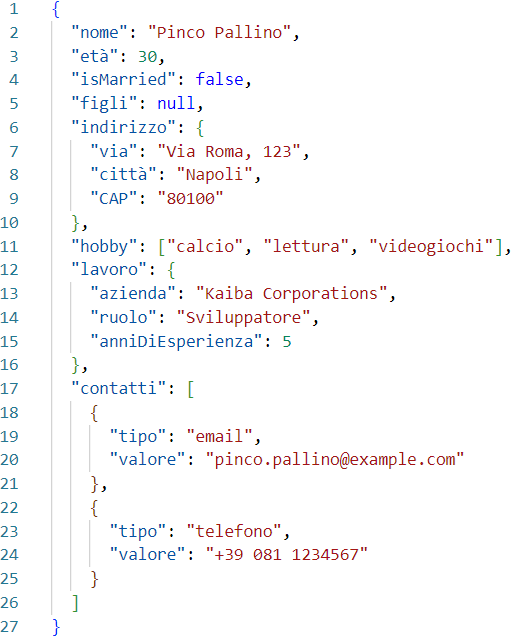
\includegraphics[keepaspectratio=true,scale=0.5]{Images/JSONExample.png}
    \caption{Esempio di oggetto JSON}
\end{figure}


Per indicare l'inizio e la fine di un oggetto vengono utilizzate le parentesi graffe (riga 1 e 27).
L'oggetto in questione utilizza la seguente rappresentazione
\begin{center}
   \emph{"chiave": valore}
\end{center}
 equiparabile ad una tavola hash o un dizionario negli ordinari linguaggi di programmazione.
 Se il valore è delimitato da virgolette allora si tratta di una stringa (riga 2), in caso contrario si tratta di un tipo primitivo (riga 3).
 Possono essere definiti anche valori nulli utilizzando la parola chiave \emph{null} (riga 5) o valori booleani (riga 4).
Inoltre è possibile rappresentare anche degli array semplici e quindi composti da singoli elementi (riga 11) oppure array complessi, nel quale ogni elemento possiede più attributi (da riga 17 a riga 26). La virgola viene utilizzata come carattere separatore degli attributi.

\thispagestyle{mystyle}

\subsection{Swagger}
\emph{Swagger} \cite{Swagger} mette a disposizione un insieme di software utili per progettare, sviluppare, documentare e testare API RESTful. Il punto saliente è la possibilità di generare una documentazione interattiva, facilitando la comprensione da parte degli sviluppatori e degli utilizzatori di tali API.
Tramite un'interfaccia grafica intuitiva, generata ad un determinato endpoint (ad esempio \emph{/api-docs}), è possibile  effettuare degli adeguati test utili a verificarne la correttezza.
Nello specifico i test di cui sopra tendono a verificare la corretta gestione delle chiamate che vengono effettuate ai server, mostrando all'utente una risposta o un eventuale errore.

La documentazione segue la specifica \textit{OpenAPI} che definisce uno standard per la documentazione delle API, in modo da renderle comprensibili, senza avere la necessità di leggere il codice sorgente.

L'insieme dei software messi a disposizione comprende:
\begin{itemize}
    \item \emph{Swagger Editor}: un editor online che permette agli sviluppatori di scrivere o modificare le API scritte seguendo le specifiche OpenAPI di cui sopra.
    \item \emph{Swagger UI}: installabile tramite npm, permette di generare una documentazione interattiva, attraverso la quale effettuare dei test.

    \item \emph{Swagger Codegen}: strumento in grado di generare in autonomia dei client \emph{SDK} (Software Development Kit) o server stubs (codice di base per i server), per permettere l'integrazione delle API nelle diverse applicazioni degli sviluppatori.

    \item \emph{Swagger Inspector}: strumento utile per testare o estrarre specifiche OpenAPI da API già esistenti.
\end{itemize}

Di seguito verrà mostrata un esempio di documentazione generata tramite swagger UI e \emph{swagger-jsdocs} per Javascript.

\begin{figure}[H]
    \centering 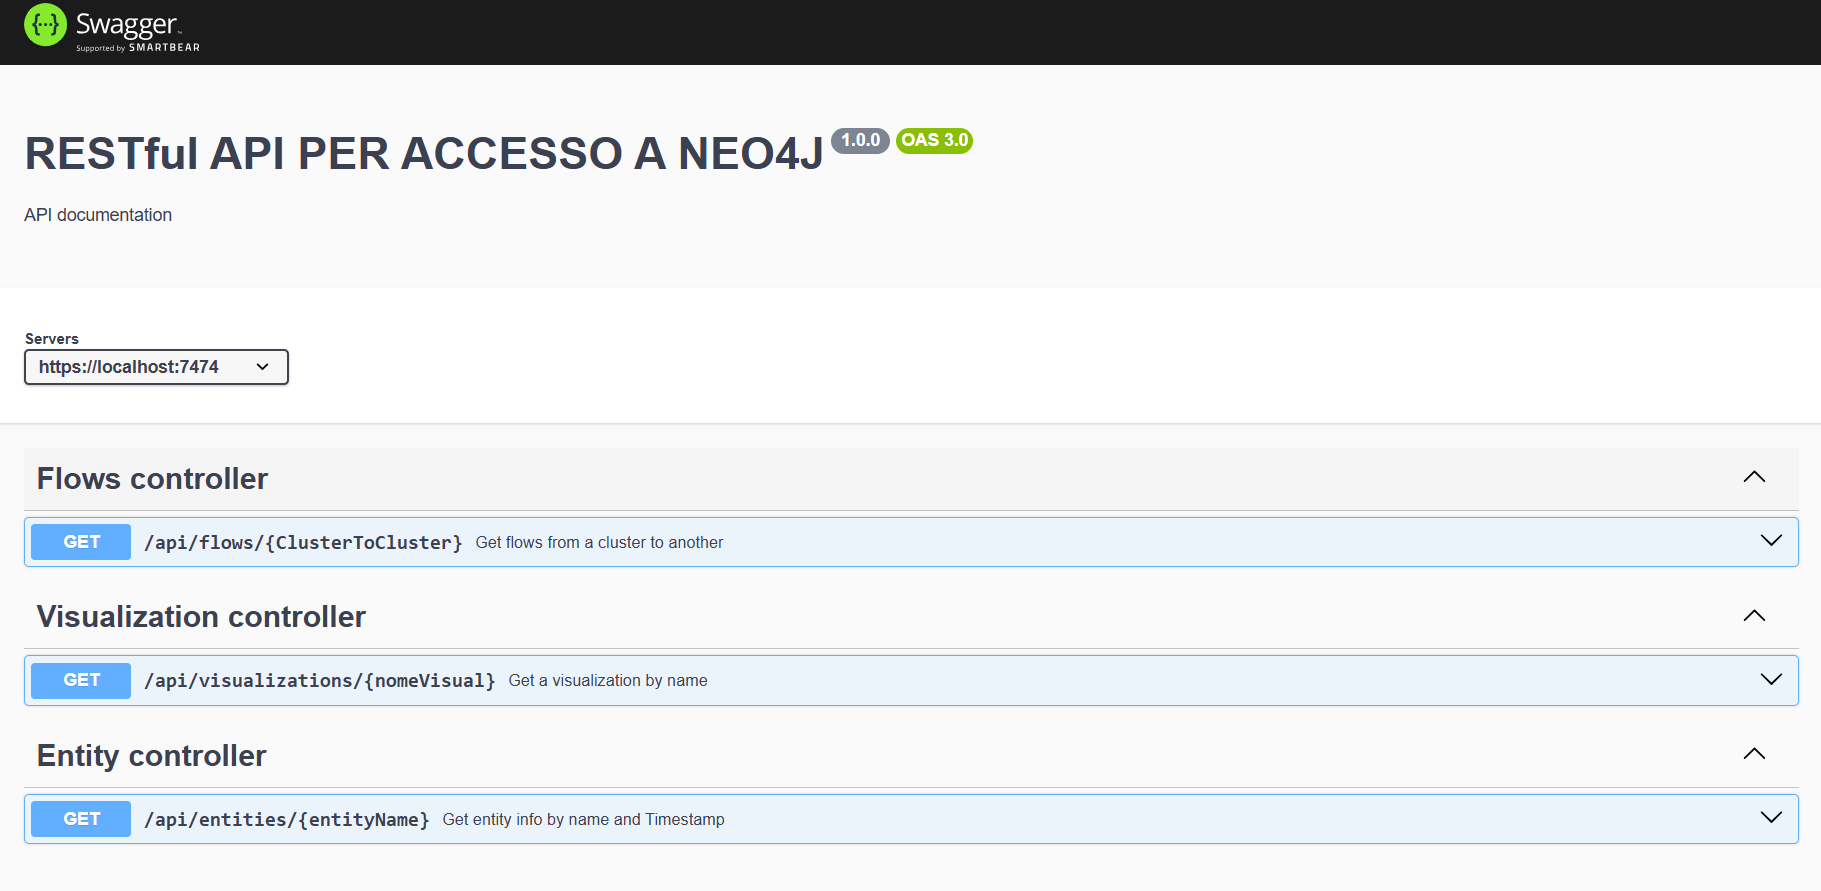
\includegraphics[keepaspectratio=true,scale=0.3]{Images/SchermataInizialeDocs.png}
    \caption{Schermata iniziale API Documentation generata con Swagger UI.}
\end{figure}

\thispagestyle{mystyle}



\end{onehalfspacing}

\clearpage

\section{Obiettivo del progetto}
\begin{onehalfspacing}

Come già accennato in precedenza, l'imponente affermazione mediatica delle blockchain ha contribuito a una crescita significativa dell'attenzione verso lo sviluppo di strumenti e software volti a migliorare l'interpretazione e l'analisi di tali strutture.
Considerata inoltre la quantità di dati presenti in quest'ultime, gli aspetti fondamentali da considerare riguardano il loro immagazzinamento e l'efficienza cui è possibile utilizzarli.

L'utilizzo dei database a grafo rappresenta una grande rivoluzione per la gestione di dati complessi, eterogenei ed interconnessi, i quali, a differenza di quelli relazionali permettono di interrogare relazioni intricate in modo più semplice e naturale, particolarmente utili nel contesto delle blockchain, dove le transazioni e le loro relazioni devono essere tracciate in modo preciso. Inoltre, offrono una soluzione più scalabile migliorando le prestazioni e aprendo nuove possbilità per l'analisi complessa dei dati, la quale necessita di un sistema di reperimento delle informazioni molto efficiente ed efficace.

L'obiettivo principale di questo progetto di tesi è quello di mettere a disposizione ai suddetti strumenti, i dati della blockchain di Bitcoin, tramite lo sviluppo di una base di dati a grafo ed un sistema di API in grado di permetterne un'estrapolazione più efficace ed efficiente.
Nonostante la possibilità di estrarre anche dati generici tramite l'API, il suo sviluppo è incentrato sull'interazione del database con un particolare sistema denominato \textit{BITVAS}.



\subsection{Cenni BITVAS}

BITVAS \cite{TesiBITVAS} è un tool di visualizzazione, sviluppato da Elisa Spigarelli con lo scopo di facilitare le analisi dei dati relativi alla blockchain di Bitcoin.
Il sistema è interattivo e permette agli utenti di selezionare specifiche informazioni tramite un'interfaccia grafica accessibile tramite browser.

Lo sviluppo di un adeguato \emph{paradigma visuale} ha reso più semplice la comprensione della  massiccia mole di dati di cui è composta la struttura dati.
Infatti, a differenza degli altri sistemi, che si concentrano su una visione d'insieme di tutta la struttura, spesso di difficile interpretazione, BITVAS si concentra sulla visualizzazione di un numero minore di dati, permettendo l'analisi di alcuni aspetti altrimenti non valutabili.

Le informazioni trattate riguardano principalmente blocchi, le transazioni e i miner.
L'attenzione è focalizzata sulle relazioni tra blocchi, presenti nella maggior parte delle visualizzazioni sviluppate, in grado di restituire informazioni riguardo i volumi di cryptovaluta scambiati in un derterminato arco temporale.
\newpage
\thispagestyle{mystyle}
\begin{figure}[H]
    \centering 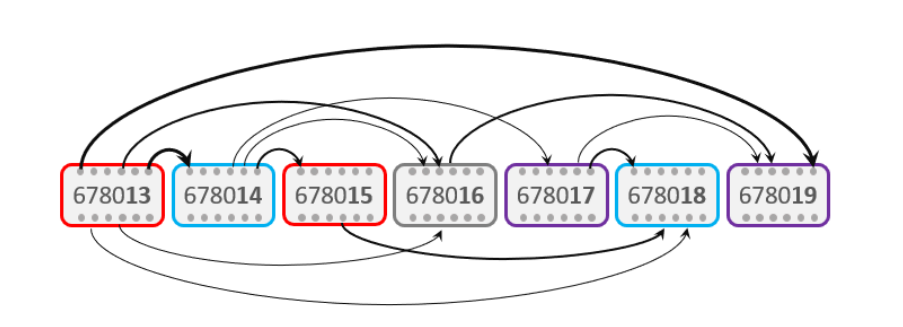
\includegraphics[keepaspectratio=true,scale=0.5]{Images/exampleBitvasVis.png}
    \caption{Visualizzazione generica BITVAS}
\end{figure}

In figura 3 è mostrato un esempio di visualizzazione adottata da BITVAS, il cui fulcro è una catena di blocchi.
Ognuno di essi è rappresentato da un rettangolo identificato da un numero che rappresenta la sua altezza nella blockchain, il cui colore del contorno sta ad indicare il miner o il mining pool che lo ha minato.
Nel caso in cui l'output di almeno una transazione all'interno di un blocco venga utilizzato come input in una transazione di un altro blocco, la relazione tra i due viene definita tramite una freccia, il cui spessore è definito dal numero di transazioni coinvolte.

Di fondamentale importanza è l'introduzione dei \emph{Cluster block}, ovvero un insieme di blocchi che vengono aggregati utili a determinate visualizzazioni, in quanto permette di rappresentare dei blocchi consecutivi dei quali non si è interessati ai dettagli.



\begin{figure}[H]
    \centering 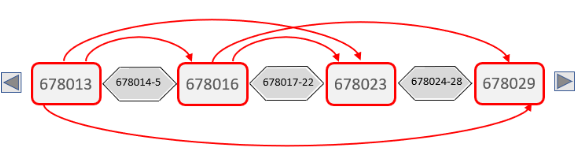
\includegraphics[keepaspectratio=true,scale=0.7]{Images/MinerVisualization2.png}
    \caption{Miner Visualization di  BITVAS}
\end{figure}

In figura 4 la visualizzazione presa in esame riguarda tutti i blocchi di un determinato arco temporale, che sono stati minati dallo stesso miner.
In questo caso i Cluster Blocks vengono utilizzati per trascurare i dettagli e le relazioni dei blocchi che non soddisfano i requisiti sopra citati. 


\subsection{Cenni al graph database di riferimento}
La crescente attenzione degli ultimi anni per le cryptovalute ha portato come conseguenza ad un aumento massiccio dei dati conservati nelle blockchain, la cui dimensione al giorno d'oggi, per quanto riguarda Bitcoin è di circa 590 Gigabyte \cite{blockchair}.
In genere, i tool di visualizzazione che prendono di mira tale mole di dati, non la utilizzano tutta, bensì applicano un filtraggio per ottenere solo quelli necessari all'adempimento delle richieste degli utenti.

Inoltre, le sole informazioni presenti nelle blockchain sono quelle riguardanti i blocchi, le transazioni e le relazioni tra essi, rappresentative dei flussi di Bitcoin, le quali possono essere limitate e in certi casi limitanti per analisi più approfondite.
Lo sviluppo del database a grafo è incentrato sulla possibilità di introdurre altri livelli di dettaglio, in grado di permettere una visione d'insieme di alcuni flussi di cryptovaluta.

L'obiettivo del database a grafo sviluppato è quello di aumentare la granularità delle informazioni presenti nella blockchain, aggregando queste ultime in cluster (ore, giorni, mesi e anni) collegati tra loro in base alle relazioni presenti ai livelli sottostanti.
In questo modo si possono reperire i flussi appartenenti ad un insieme di blocchi.
Questo approccio non solo migliora la comprensione dei flussi di cryptovaluta, ma riduce anche il carico computazionale necessario per l’estrazione delle informazioni, rendendo il processo di analisi più veloce e meno oneroso.

Inoltre, l’uso di un database a grafo permette di identificare pattern e anomalie nei flussi di criptovaluta che potrebbero non essere evidenti con un’analisi tradizionale. Ad esempio, è possibile tracciare il movimento di grandi quantità di Bitcoin tra diversi indirizzi, identificando potenziali attività sospette o comportamenti di mercato significativi. Questo livello di analisi avanzata è fondamentale per migliorare la sicurezza e la trasparenza delle transazioni in criptovaluta.

\thispagestyle{mystyle}





\end{onehalfspacing}

\clearpage
\section{Progetto ed implementazione dell'API}
\begin{onehalfspacing}
  In questo capitolo viene presentato un excursus sulle varie fasi della progettazione e implementazione del database a grafo e dell'API RESTful. 
Per quanto riguarda la base di dati, ne viene descritta la struttura e ne vengono evidenziati i vantaggi. Inoltre vengono mostrate alcune delle query più importanti per l'implementazione del database, come quelle legate alla definizione delle relazioni tra le entità, oppure quelle utili al reperimento di dati, ad esempio quelli utilizzati dalle visualizzazioni di BITVAS.

L'approccio della trattazione dell'API è di tipo top-down, partendo con la definizione dell'architettura e del diagramma di comunicazione tra i vari moduli progettati, fino agli endpoint messi a disposizione dalla API e di conseguenza le funzionalità sviluppate.
Infine vengono descritti in modo più specifico i singoli moduli, evidenziandone tutte le particolarità.

\subsection{Struttura del Database}

Le entità principali delle visualizzazioni messe a disposizione da BITVAS sono quindi i flussi di Bitcoin tra blocchi o transazioni.
Questi ultimi sono oggetto di studi in diversi campi, partendo dalla cybesecurity, attraverso l'individuazione e la prevenzione di possibili pattern malevoli, fino ad arrivare a studi speculativi sul prezzo di Bitcoin.

L'analisi dei \emph{tempi di permanenza} (o in inglese \emph{holding time}) dei bitcoin all'interno dei portafogli degli utenti della rete \cite{holdingTimes} è uno degli aspetti fondamentali per questi tipi di valutazione, tramite i quali è possibile catalogare i vari tipi di holders.
Nonostante la necessità del supporto di strumenti statistici per comprenderne tutti i dettagli e le relazioni che li legano, la possibilità di sviluppo di altre visualizzazioni per BITVAS, in grado di dare un'anteprima visuale su tali holding times e il bisogno di semplificare l'interpretazione della grande mole di dati presenti nella blockchain, ha portato allo sviluppo della seguente base di dati a grafo, tramite la quale è possibile gestire il gran numero di relazioni tra le informazioni in modo più efficiente ed efficace.
\newpage
\thispagestyle{mystyle}
\begin{figure}[H]
    \centering 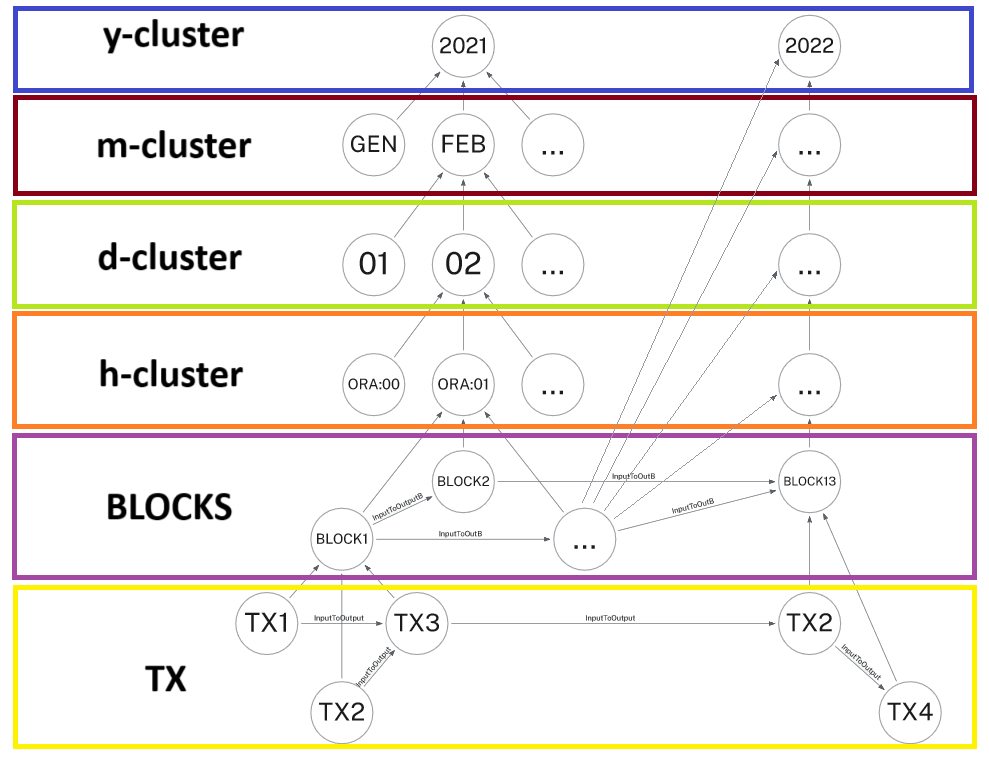
\includegraphics[keepaspectratio=true,scale=0.58]{Images/ExampleDB.png}
    \caption{Rappresentazione concettuale ed estesa del database a grafo}
\end{figure}

In figura 5 è rappresentato il database di riferimento.
La struttura è di tipo \emph{time-tree} (in italiano, albero temporale), alla cui base si trovano le entità fondamentali corrispondenti a quelle utilizzate nella blockchain di Bitcoin, ovvero blocchi e transazioni.
Ognuna delle quali possiede attributi in grado di fornirne i dettagli, tra cui quelli utilizzati per la loro identificazione univoca, come \textit{id} per blocchi o \textit{hash} per le transazioni.

Come già trattato, la blockchain al giorno d'oggi fa riferimento ad una grande quantità di informazioni, legati anche ai flussi di Bitcoin.
Per rendere più efficiente l'estrapolazione dei dati nei casi in cui si voglia tener conto di flussi che partono o arrivano ad un determinato insieme di blocchi, appartenenti ad un definito arco temporale ed evitare un'analisi dispendiosa  al livello di blocco o transazione, si è deciso di progettare più livelli di clusterizzazione.

Il livello successivo ai blocchi è dato dagli \emph{h-cluster} (hour-cluster), che fanno riferimento ai blocchi minati in una determinata ora, ovvero circa sei.
Salendo nella struttura si incontrano, nel seguente ordine, i \emph{d-cluster} (day-cluster), \emph{m-cluster} (month-cluster) e \emph{y-cluster} (year-cluster).

Il tipo di struttura, in grado di facilitare la ricerca tramite \emph{timestamp}, è definita dalle relazioni gerarchiche,
nel caso in cui un nodo di livello inferiore faccia parte di uno dei cluster superiori.
Un esempio di relazione gerarchica è quella tra transazioni e blocchi o tra blocchi e h-cluster. 
Con l'utilizzo di attributi come \emph{minimum} e \emph{maximum}, che rappresentano rispettivamente l'id minimo e massimo dei blocchi a cui fa riferimento il cluster, anche la ricerca tramite id viene valorizzata dal database.
Inoltre per facilitare il reperimento dei flussi di Bitcoin che riguardano cluster di livello diverso, ognuno di essi, all'occorrenza, ha una relazione con tutti gli altri cluster verso il quale spende Bitcoin, la quale contiene informazioni riguardante il volume di valuta scambiato, attraverso due parametri, ovvero \emph{value} e \emph{value$\_$usd}.

Di seguito viene mostrato il modello completo della base di dati, con tutti i nodi e le relazioni presenti al suo interno.

\thispagestyle{mystyle}

\begin{figure}[H]
    \centering 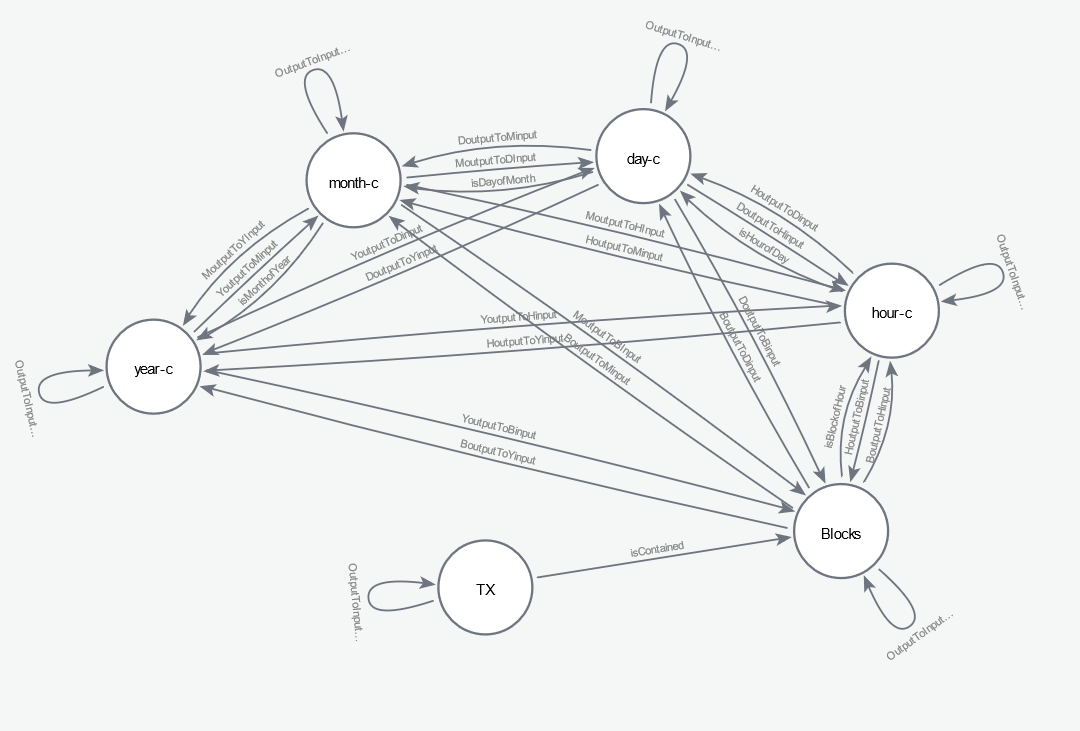
\includegraphics[keepaspectratio=true,scale=0.52]{Images/Modello completo.png}
    \caption{Modello completo del database a grafo}
\end{figure}
Per evidenziare il collegamento di una transazione con un blocco viene fatto riferimento alla relazione \emph{isContained}, mentre per le altre gerarchie viene utilizzato lo schema nominativo \emph{isXofY}.
I flussi di Bitcoin invece sono definiti dalle relazioni \emph{XOutputToYInput}.
Per entrambi i tipi, al posto di X e Y vanno sostituiti i cluster a cui si fa riferimento.
Se un flusso si riferisce a due nodi appartenenti alla stessa tipologia di nodo, la nomenclatura utilizzata è \emph{OutputToInputX}.
Ad esempio per i blocchi la relazione che identifica i flussi è \emph{OutputToInputB}.
Le relazioni che partono e arrivano alla stesso nodo si riferiscono agli scambi di cryptovaluta che avvengono nello stesso arco temporale definito dal cluster di riferimento.
Ad esempio una autorelazione di un blocco, sta ad indicare la presenza di un flusso di Bitcoin tra due transazioni validate al suo interno.

Il database implementato prevede all'incirca due milioni e mezzo di nodi e quattro milioni di relazioni, strutturate come segue:



\begin{center}
\begin{tabular}{|c|c|c|}
\hline
 LISTA BLOCCHI & LISTA TRANSAZIONI & FILE INPUT.CSV \\ 
 \hline
 2023-12-07 & 2023-12-07 & 2023-12-20 \\ 
  to & 2023-12-18 & 2024-01-05 \\
  2024-01-07 & 2023-12-20 & \\
   & 2024-01-04 & \\
   & 2024-01-05 & \\
 \hline
\end{tabular}

\end{center}
\thispagestyle{mystyle}
L'insieme dei dati è stato estrapolato dal dataset messo a disposizione su Blockchair.com \cite{blockchair}. I file INPUT.CSV sono quelli utili per la definizione delle relazioni che rappresentano i flussi di Bitcoin.

\subsubsection{Query per la definizione della struttura}
Di seguito vengono mostrate le Cypher Query più importanti utilizzate per la definizione della struttura della base di dati.

\begin{center}
Creazione dei nodi Transaction
   \begin{lstlisting}

            LOAD CSV WITH HEADERS FROM 'file:///TX.csv'
            AS row WITH split(row.time,' ')AS date, row
            MERGE (:Transaction {block_id: row.block_id, 
                   hash: row.hash,
                   input_count: row.input_count,
                   output_count: row.output_count, 
                   input_total: row.input_total, 
                   input_total: row.input_total,  
                   output_total: row.output_total, 
                   fee: row.fee,
                   is_coinbase: row.is_coinbase})
\end{lstlisting} 
\end{center}
Con i dati presenti nel file TX.csv vengono inizializzati i nodi che rappresentano le transazioni all'interno della base di dati, con i relativi attributi.
\newpage \thispagestyle{mystyle}
\begin{center}
Creazione dei nodi Blocks
   \begin{lstlisting}

            LOAD CSV WITH HEADERS FROM 'file:///Blocchi.csv'
            AS row WITH split(row.time, ' ') AS date ,row
            MERGE (:Blocks {id: row.id, hash: row.hash, 
                    time:   datetime(date[0]+'T'+date[1]+'Z'),
                    transaction_count: row.transaction_count, 
                    input_count: row.input_count, 
                    output_count: row.output_count,
                    input_total: row.input_total,  
                    output_total: row.output_total, 
                    fee_total: row.fee_total,
                    guessed_miner: row.guessed_miner})
\end{lstlisting} 
\end{center}
 Con questa query vengono inseriti i nodi rappresentativi dei blocchi all'interno del database con i relativi attributi estratti dal file Blocchi.csv.
 
 Per la costruzioine delle relazioni tra transazioni e blocchi, e quindi generare una sorta di grafo delle transazioni, vengono utilizzate le seguenti query, che usufruiscono dei dati presenti nei file INPUT.csv.

\vspace{5mm}
\begin{center}
Creazione delle relazioni tra blocchi
   \begin{lstlisting}

            LOAD CSV WITH HEADERS FROM 'file:///IN_20240105.csv' AS row
            MATCH (b:Blocks {id:row.block_id}), 
                  (b2:Blocks {id:row.spending_block_id})
            MERGE  (b)-[ib:inputToOutputB]->(b2)
            SET (ib.block_id=row.block_id, 
                ib.spending_block_id=row.spending_block_id, 
                ib.value=row.value,
                ib.is_from_coinbase = row.is_from_coinbase, 
                ib.is_spendable= row.is_spendable, 
                ib.value_usd = row.value_usd)
\end{lstlisting} 
\end{center}
\newpage \thispagestyle{mystyle}
\begin{center}
Creazione delle relazioni tra transazioni
\begin{lstlisting}

            LOAD CSV WITH HEADERS FROM 'file:///IN_20240105.csv' AS row
            MATCH (t:Transactions {hash:row.transaction_hash}), 
                  (t2:Transactions{hash:row.spending_transaction_hash})
            MERGE  (t)-[i:inputToOutputTX]->(t2)
            SET i.transaction_hash=row.transaction_hash,
                i.spending_TX_hash=row.spending_TX_hash,
                i.value=row.value,
                i.value_usd = row.value_usd,
                i.is_from_coinbase = row.is_from_coinbase
\end{lstlisting} 
\end{center}
 Nelle seguenti query viene mostrata la definizione degli altri cluster progettati a partire dall'attributo time dei nodi appena inseriti, estrapolandone le porzioni necessarie (es. per i day-cluster vengono estratti anno,mese e giorno).
\vspace{5mm}
\begin{center}
Creazione dei nodi Hour-Cluster
   \begin{lstlisting}

            MATCH(b:Blocks)  
            WITH DISTINCT (b.time.year 
                            + '-' + b.time.month 
                            + '-' + b.time.day 
                            + 'T' + b.time.hour) AS IDHour
            CREATE (h:hCluster{htime:IDHour})
\end{lstlisting} 
\end{center}
\vspace{3mm}
 \begin{center}
Creazione dei nodi Day-Cluster

   \begin{lstlisting}
            MATCH(b:Blocks)  
            WITH DISTINCT (b.time.year 
                            + '-' + b.time.month 
                            + '-' + b.time.day) AS IDDay
            CREATE (d:dCluster{dtime:IDDay})
\end{lstlisting} 
\end{center}

\newpage \thispagestyle{mystyle}

 \begin{center}
Creazione dei nodi Month-Cluster
   \begin{lstlisting}

            MATCH(b:Blocks)  
            WITH DISTINCT (b.time.year 
                            + '-' + b.time.month) AS IDMonth
            CREATE (m:mCluster{mtime:IDMonth})
\end{lstlisting} 
\end{center}
\vspace{2mm}
\begin{center}
Creazione dei nodi Year-Cluster
   \begin{lstlisting}

            MATCH(b:Blocks)  
            WITH DISTINCT (b.time.year) AS IDYear
            CREATE (y:yCluster{ytime:IDYear})
\end{lstlisting} 
\end{center}


Dopo aver definito tutte le entità appartenenti alla base di dati, sono state definite le relazioni gerarchiche che legano i vari cluster e successivamente gli attributi di questi ultimi. Le strutture di quest'ultime sono molto simili tra loro con qualche piccola differenza in base al cluster a cui si fa riferimento. Di seguito sono mostrate le query usate per la gestione degli Hour-Cluster.

\vspace{5mm}
\begin{center}
Creazione relazioni tra blocchi e Hour-Cluster
\begin{lstlisting}

            MATCH (b:Blocks),(h:hCluster)  
            WHERE h.htime = b.time.year 
                    + '-' + b.time.month
                    + '-' + b.time.day 
                    + 'T' + b.time.hour
                    
            MERGE (b)-[i:isBofH]->(h)
\end{lstlisting} 
\end{center}
\vspace{2mm}
\begin{center}
Inizializzazione attributi degli Hour-Cluster
\begin{lstlisting}

            MATCH (b:Blocks)-[r:isBofH]->(h:hCluster) 
            WITH DISTINCT h,
                    sum(toInteger(b.input_total)) AS total_h_input,
                    sum(toInteger(b.output_total)) AS total_h_output

            MERGE (b)-[i:isBofH]->(h)
\end{lstlisting} 
\end{center}
\newpage \thispagestyle{mystyle}
In seguito alla definizione di tutti i cluster e delle relazioni gerarchiche, la struttura del database assume la forma di un albero temporale, tramite il quale le query di ricerca tramite timestamp risultano molto efficaci.
Le query per l'inizializzazione delle relazioni identificative dei flussi di Bitcoin sono di due tipi, quelle riguardanti lo stesso tipo di cluster o meno.
Quest'ultime hanno una struttura molto simile per ogni cluster.
Di seguito vengono mostrate quelle utilizzate per la creazione di quelle riguardanti i flussi il cui punto di partenza sono gli Hour-Cluster.
\vspace{5mm}
\begin{center}
Inizializzazione relazioni tra i nodi Hour-Cluster
\begin{lstlisting}

           MATCH (b:Blocks)-[ih:isBofH]->(h:hCluster),
                    (b2:Blocks)-[ih2:isBofH]->(h2:hCluster), 
                    (b)-[ib:inputToOutputB]->(b2)
            WITH DISTINCT h,h2,sum(toInteger(ib.value))AS hClusterFlow, 
                          sum(toFloat(ib.value_usd))AS hClusterFlowUSD
                          
            MERGE (h)-[ih:inputToOutputH]->(h2)
            SET ih.value = hClusterFlow,
                ih.value_usd = hClusterFlowUSD

\end{lstlisting} 
\end{center}

\vspace{5mm}
\begin{center}
Inizializzazione relazioni tra Hour-Cluster e Year-Cluster
\begin{lstlisting}

            MATCH (h2:hCluster)-[io:inputToOutputH]->
                    (h:hCluster)-[ih:isHofD]->
                    (d:dCluster)-[id:isDofM]->
                    (m:mCluster)-[i:isMofY]->
                    (y:yCluster) 
            WITH h2,y,sum(io.value) AS value, 
                 sum(io.value_usd) AS value_usd
                
            MERGE (h2)-[ib:HOutputToYInput]->(y)
            SET ib.value = value, 
                ib.value_usd = value_usd

\end{lstlisting} 
\end{center}

\vspace{5mm}
\newpage \thispagestyle{mystyle}
\begin{center}
Inizializzazione relazioni tra Hour-Cluster e Blocks
\begin{lstlisting}

            MATCH (b2:Blocks)-[io:inputToOutputB]->
                  (b:Blocks)-[iblock:isBofH]->(h:hCluster),
                  (b2)-[iblock2:isBofH]->(h2:hCluster)
            WHERE b2.time <> b.time
            WITH h2,b,io,sum(io.value) AS value,
                 sum(io.value_usd) AS value_usd
                
            MERGE (h2)-[ioy:HOutputToBInput]->(b)
            SET  ioy.value = value, 
                 ioy.value_usd = value_usd

\end{lstlisting} 
\end{center}
\vspace{3mm}
\begin{center}
Inizializzazione relazioni tra Hour-Cluster e Day-Cluster
\begin{lstlisting}

            MATCH (h2:hCluster)-[io:inputToOutputH]->
                  (h:hCluster)-[ih:isHofD]->(d:dCluster)
            WITH h2,d,sum(io.value) AS value, 
                 sum(io.value_usd) AS value_usd

            MERGE (h2)-[ib:HOutputToDInput]->(d)
            SET ib.value = value, 
                ib.value_usd = value_usd

\end{lstlisting} 
\end{center}

\vspace{3mm}
\begin{center}
Inizializzazione relazioni tra Hour-Cluster e Month-Cluster
\begin{lstlisting}

            MATCH (h2:hCluster)-[io:inputToOutputH]->
                  (h:hCluster)-[ih:isHofD]->
                  (d:dCluster)-[id:isDofM]->(m:mCluster)
            WITH h2,m,sum(io.value) AS value, 
                 sum(io.value_usd) AS value_usd

            MERGE (h2)-[ib:HOutputToMInput]->(m) 
            SET ib.value = value, 
                ib.value_usd = value_usd
\end{lstlisting} 
\end{center}
\newpage \thispagestyle{mystyle}
Per permettere la ricerca dei blocchi anche tramite id e non solo tramite timestamp, sono stati aggiunti due parametri ai cluster, ovvero minimum e maximum che indicano rispettivamente l'id minimo e massimo a cui fa riferimento.
Questi vengono definiti con le seguenti query.

\vspace{3mm}
\begin{center}
Inizializzazione minimum e maximum per gli Hour-Cluster
\begin{lstlisting}

            MATCH (b:Blocks)-[r:isBofH]->(h:hCluster)
            WITH  h,
                  MIN(b.id)AS MINIMUM,
                  MAX(b.id) AS MAXIMUM
                  
            SET   h.mimimum = MINIMUM,
                  h.maximum = MAXIMUM
\end{lstlisting} 
\end{center}

\vspace{3mm}
\begin{center}
Inizializzazione minimum e maximum per i Day-Cluster
\begin{lstlisting}

            MATCH (h:hCluster)-[r:isHofD]->(d:dCluster)
            WITH  d,
                  MIN(h.minimum)AS MINIMUM,
                  MAX(h.maximum) AS MAXIMUM
                  
            SET   d.mimimum = MINIMUM,
                  d.maximum = MAXIMUM
\end{lstlisting} 
\end{center}

Le query per la definizione di questi attributi per gli altri cluster sono uguali a quest'ultima con adeguato adattamento delle entità prese come riferimento.

\subsubsection{Query per il reperimento di dati}
La struttura generata assume di conseguenza la forma di un time-tree i cui nodi sono legati da relazioni che rappresentano i flussi di Bitcoin, tramite la quale è possibile etrarre i dati necessari per le visualizzazioni di BITVAS e non solo, in maniera semplice, veloce ed efficace.
Infatti la ricerca di un determinato nodo tramite timestamp, o id nel caso dei blocchi risulta fortemente migliorata, in quanto non è necessaria la verifica di tutti i nodi,ma viene effettuata seguendo la struttura ad albero. 
Di seguito vengono mostrate le query utilizzate dall'API per permettere un'interazione con il database.

\newpage \thispagestyle{mystyle}

\begin{center}
Flussi tra Day-Cluster
\begin{lstlisting}

            MATCH (d:dCluster)-[im:isDofM]->
                  (m:mCluster)-[iy:isMofY]->(y:yCluster)
            WHERE y.ytime = '2024' AND m.mtime = '2024-01'
                  AND d.dtime = '2024-01-05'
            WITH d

            MATCH (d2)-[io:inputToOutputD]->(d)
            WHERE d2.dtime >= '2023-12-10' 
                  AND d2.dtime <='2023-12-20' 
            RETURN d2.dtime,d.dtime,io.value,io.value_usd
\end{lstlisting} 
\end{center}

La prima parte della query permette di individuare il cluster di arrivo attraverso la struttura ad albero, il quale viene utilizzato successivamente per selezionare tutti i flussi che arrivano ad esso e che partono da un insieme di day-cluster definiti tramite un arco temporale ben definito.

\vspace{5mm}
\begin{center}
Flussi da Hour-Cluster a Day-Cluster 
\begin{lstlisting}

            MATCH (d:dCluster)-[id:isDofM]->
                  (m:mCluster)-[im:isMofY]->(y:yCluster)
            WHERE y.ytime = '2024' 
                  AND m.mtime = '2024-01' 
                  AND d.dtime='2024-01-05'
            WITH d

            MATCH (h:hCluster)-[rels:HOutputToDInput]->(d)
            WHERE h.htime >='2023-12-10T02' 
                  AND h.htime <= '2023-12-20T04' 
            RETURN  h.htime,rels.value,rels.value_usd,d.dtime
\end{lstlisting} 
\end{center}

In questo caso vengono prelevati tutti i flussi che hanno come punto di partenza gli hour-cluster definiti dall'arco temporale scelto e come punto di arrivo il day-cluster selezionato.

Oltre a query strettamente legate ai flussi di Bitcoin è possibile anche prelevare gli attributi delle entità all'interno del database e quindi ottenere delle informazioni generali. In seguito viene mostrato un esempio di quest'ultime.

\newpage \thispagestyle{mystyle}

\begin{center}
Ottenimento informazioni dei blocchi
\begin{lstlisting}

            MATCH (b:Blocks)-[i:isBofH]->
                  (h:hCluster)-[ih:isHofD]->
                  (d:dCluster)-[id:isDofM]->
                  (m:mCluster)-[im:isMofY]->(y:yCluster)
            WHERE y.ytime = '2024'  
                  AND m.mtime = '2024-01' 
                  AND d.dtime = '2024-01-05' 
                  AND h.htime = '2024-01-05T02'
                  AND b.time = '2024-01-05T02:47:03'
            RETURN b.id,toString(b.time),b.hash,
                   b.guessed_miner,b.fee_total,
                   b.output_count,b.input_count,b.output_total,
                   b.input_total, b.transaction_count 
                   ORDER BY b.time
\end{lstlisting} 
\end{center}
\vspace{5mm}
\begin{center}
Ottenimento informazioni dei Month-Cluster
\begin{lstlisting}

            MATCH MATCH (m:mCluster)-[im:isMofY]->(y:yCluster)
            WHERE y.ytime = '2024'  
                  AND m.mtime = '2024-01'
            RETURN m.mtime,m.minimum,m.maximum,
                   m.total_m_input,m.total_m_output
                   ORDER BY m.mtime
\end{lstlisting} 
\end{center}

La struttura della query per l'estrazione dei dati riguardanti gli altri cluster è pressochè identica.
Si parte con l'individuazione tramite la struttura ad albero, dopodichè si estraggono i corrispondenti dati.

Come trattato in precedenza il focus dello sviluppo dell'API e del database si basa sull'interazione di quest'ultimo con BITVAS. Di seguito vengono mostrate le query utili al reperimento dei dati per le visualizzazioni già esistenti.

\newpage \thispagestyle{mystyle}

\begin{center}
Ottenimento prima parte della BlockVisualization
\begin{lstlisting}

            WITH datetime('2024-01-05T09:43:19Z') - duration('PT12H') 
                 AS firstTwelveT
            MATCH  (b:Blocks)-[i:isBofH]->
                   (h:hCluster)-[ih:isHofD]->
                   (d:dCluster)-[id:isDofM]->
                   (m:mCluster)-[im:isMofY]->(y:yCluster)
            WHERE y.ytime = '2024' AND m.mtime ='2024-01'  
                  AND d.dtime ='2024-01-05' 
                  AND h.htime  = '2024-01-05T09' 
                  AND b.time=datetime('2024-01-05T09:43:19Z')
            With b, firstTwelveT
            
            MATCH (h)-[i:inputToOutputB]->(b)
            WHERE h.time >= firstTwelveT AND h.time<= b.time
            RETURN h.id,h.time,b.id,b.time ORDER BY h.time
\end{lstlisting} 
\end{center}
La BlockVisualization pone il focus su un determinato blocco e i flussi di Bitcoin che arrivano e partono da esso.
In questo caso vendono estrapolati i dati identificativi dei flussi che partono da blocchi il cui timestamp è compreso nelle dodici ore precedenti e arrivano blocco scelto.

\begin{center}
Ottenimento seconda parte della BlockVisualization
\begin{lstlisting}
            WITH datetime('2024-01-05T09:43:19Z') + duration('PT12H') 
                 AS secondTwelveT
            MATCH  (b:Blocks)-[i:isBofH]->
                   (h:hCluster)-[ih:isHofD]->
                   (d:dCluster)-[id:isDofM]->
                   (m:mCluster)-[im:isMofY]->(y:yCluster)
            WHERE y.ytime = '2024' AND m.mtime ='2024-01'  
                  AND d.dtime ='2024-01-05' 
                  AND h.htime  = '2024-01-05T09' 
                  AND b.time=datetime('2024-01-05T09:43:19Z')
            With b, secondTwelveT 
            
            MATCH (b)-[i:inputToOutputB]->(h) 
            WHERE h.time <= secondTwelveT AND h.time > b.time  
            RETURN b.id,b.time,h.id,h.time ORDER BY h.time
\end{lstlisting} 
\end{center}
\newpage \thispagestyle{mystyle}
La struttura è molto simile alla prima, con qualche piccola diffenza legata al punto di partenza dei flussi, che in questo caso è il blocco centrale della visualizzazione. Mentre il punto di arrivo sono i blocchi il cui timestamp è compreso nelle dodici ore successive al blocco selezionato.
L'insieme delle due permettono l'estrapolazione necessaria per ottenere l'intera visualizzazione.

Anche la TransactionVisualization `e divisa in due parti, mostrate di seguito.
\begin{center}
Ottenimento prima parte della Transaction Visualization
\begin{lstlisting}
            WITH  hash AS chosenTX
            MATCH (t:Transactions)
            WHERE t.hash = chosenTX
            WITH t

            MATCH (t)-[r:inputToOutputTX]->(c)
            RETURN t.hash as hash, t.block_id as blockStart, 
                   c.hash as hashEnd, c.block_id as blockEnd, 
                   r.value as value, r.value_usd as value_usd 
                   ORDER BY c.block_id
\end{lstlisting} 
\end{center}
\vspace{5mm}
\begin{center}
Ottenimento seconda parte della TransactionVisualization
\begin{lstlisting}
            WITH  hash AS chosenTX
            MATCH (t:Transactions)
            WHERE t.hash = chosenTX
            WITH t

            MATCH (c)-[r:inputToOutputTX]->(t)
            RETURN t.hash as hash, t.block_id as blockStart, 
                   c.hash as hashEnd, c.block_id as blockEnd, 
                   r.value as value, r.value_usd as value_usd 
                   ORDER BY c.block_id
\end{lstlisting} 
\end{center}
Una volta identificata la transazione, tramite hash, all'interno del database, si individuano le relazioni che partono e arrivano ad essa corrispondenti ai flussi di Bitcoin in ingresso e in uscita.

Per quanto riguarda la MinerVisualization e la CombinedVisualization per l'estrapolazione dei blocchi da visualizzare viene utilizzata un'interrogazione che può essere identificata come `Query di ricerca' mostrata di seguito.
\newpage \thispagestyle{mystyle}
\begin{center}
Query di ricerca
\begin{lstlisting}[basicstyle = \small]
            WITH toString(datetime('2024-01-05T09:43:19Z') 
                    - duration('PT12H')) AS firstTwelveT,
                 toString( datetime('2024-01-05T09:43:19Z') 
                 + duration('PT12H')) AS secondTwelveT
            WITH  split(firstSplit[0],'-') AS firstDate,
                  split(firstSplit[1],':') AS firstTime,
                  split(secondSplit[0],'-') AS secondDate,
                  split(secondSplit[1],'-') AS secondTime
                  
            MATCH  (b:Blocks)-[i:isBofH]->
                   (h:hCluster)-[ih:isHofD]->
                   (d:dCluster)-[id:isDofM]->
                   (m:mCluster)-[im:isMofY]->(y:yCluster)
            WHERE  y.ytime >= firstDate[0] AND y.ytime <= secondDate[0] 
                   AND m.mtime >= firstDate[0] + '-' + firstDate[1] 
                   AND m.mtime <= secondDate[0] + '-' + secondDate[1] 
                   AND d.dtime >= firstDate[0] + '-' + firstDate[1] 
                                  + '-' + firstDate[2]
                   AND  d.dtime <= secondDate[0] + '-' + secondDate[1] 
                                  + '-' + secondDate[2]
                   AND  h.htime >= firstDate[0] + '-' + firstDate[1] 
                                    + '-' + firstDate[2] +'T'+ 
                                    firstTime[0]
                   AND h.htime <= secondDate[0] + '-' + secondDate[1] 
                                    + '-' + secondDate[2] + 'T' + 
                                    secondTime[0]
                   AND b.time >= (datetime('2024-01-05T09:43:19Z') 
                                - duration('PT12H'))
                   AND b.time<= ( datetime('2024-01-05T09:43:19Z') 
                                + duration('PT12H'))
            WITH collect(b) as blocchi, collect(ID(b)) as listBlocks
\end{lstlisting} 
\end{center}

Tramite quest'ultima vengono estratti tutti i blocchi il cui timestamp è compresto nelle dodici ore precedenti e successive al timestamp del blocco centrale alla visualizzazione.
Per la MinerVisualization c'è una leggera differenza, ovvero un vincolo sul miner oltre a quelli temporali.
Le collezioni di blocchi ricavate vbengono utilizzate nella successiva subquery per l'estrapolazione dei flussi.
\newpage \thispagestyle{mystyle}

\begin{center}
Estrapolazione flussi tra i blocchi estratti per la MinerVisualization e la BlockVisualization
\begin{lstlisting}
           CALL{
                  WITH blocchi,listBlocks
                  UNWIND blocchi as x
                  MATCH (x)-[r:inputToOutputB]->(c)
                  WHERE ID(c) in listBlocks
                  RETURN x,c
            }
            RETURN x.id,x.time,c.id,c.time

\end{lstlisting} 
\end{center}

\subsection{Struttura dei JSON} 
Per la definizione delle visualizzazioni implementate in BITVAS si fa uso di file JSON, adeguatamente strutturati ai fini di ognuna di esse.
La corretta comprensione di questi ultimi è necessaria per garantire la corretta interazione tra BITVAS e il database a grafo, messa in atto dall'API RESTful sviluppata.

\begin{figure}[H]
    \centering 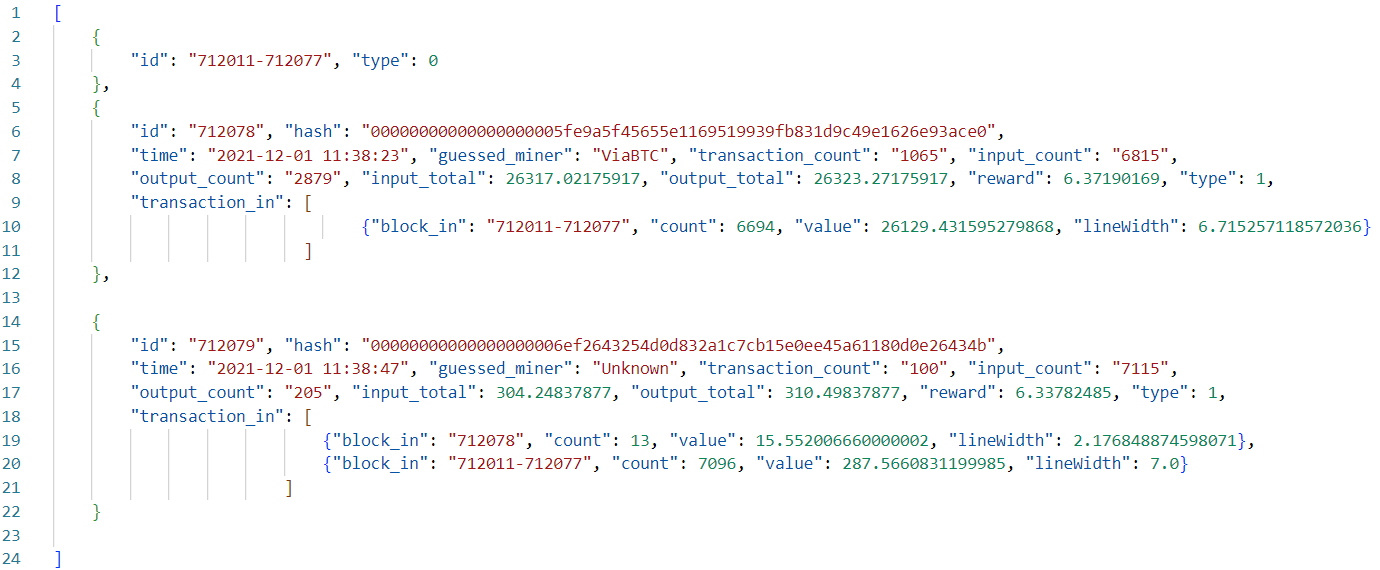
\includegraphics[keepaspectratio=true,scale=0.4]{Images/StrutturaJSON_BITVAS.png}
    \caption{Struttura del JSON usato da BITVAS per la visualizzazione iniziale}
\end{figure}

La totalità delle visualizzazioni di BITVAS pone il focus sui flussi di Bitcoin dei blocchi o delle transazioni visualizzate.
Ogni elemento del file corrisponde ad un'entità rappresentata dal software, la cui differenziazione viene gestita tramite il parametro \emph{type}, il quale può essere inizializzato con tre interi, ovvero zero, uno e due che indicano rispettivamente i cluster block, blocchi e transazioni.
In figura 7 vengono mostrate solo le prime due entità elencate.
I cluster block sono identificati da un id che contiene il range dei blocchi da cui è formato e da type.
Invece per quanto riguarda i blocchi, oltre all' id, vengono inizializzati una serie di parametri utili a fornire dettagli su di essi, tra cui \textit{guessed$\_$miner} utilizzato per identificare il miner che lo ha validato, oppure \textit{transaction$\_$count} che tiene conto del numero di transazioni validate in esso.
Inoltre per ognuno di essi è definito l'array \textit{transaction$\_$in} contenente una lista di blocchi da cui partono i flussi di bitcoin a loro legati (righe 9-11 e 18-21). 

\thispagestyle{mystyle}
La stessa struttura viene utilizzata anche quando vengono rappresentate le transazioni. In questo caso però, le relazioni visualizzate dipendono dalla transazione presa in esame, per questo motivo nel file JSON che segue il riferimento alla transazione di arrivo non è presente.

\begin{figure}[H]
    \centering 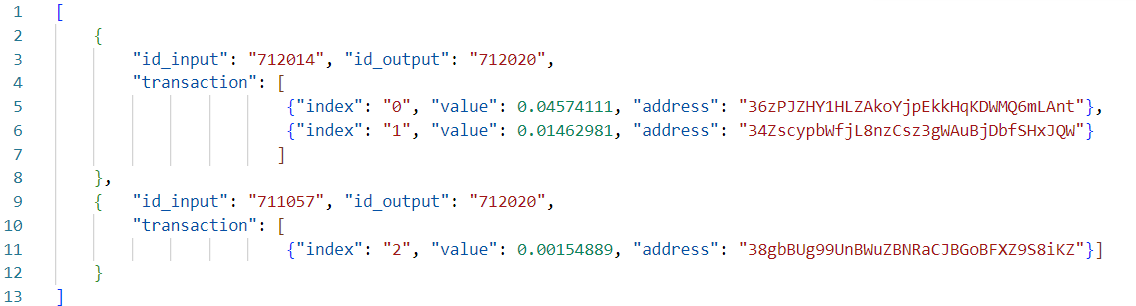
\includegraphics[keepaspectratio=true,scale=0.5]{Images/TX_JSON_BITVAS.png}
    \caption{Struttura del JSON usato per la rappresentazione delle Transazioni}
\end{figure}

\textit{id$\_$input} e \textit{id$\_$output} indicano il blocco di partenza e di arrivo del flusso legato alla transazione selezionata tramite interaccia grafica.
Le transazioni coinvolte in tale flusso sono identificate dall'array \textit{transaction}.

Infine per comprendere l'appartenenza di una transazione ad un determinato blocco, il sistema utilizza la struttura mostrata di seguito.


\begin{figure}[H]
    \centering 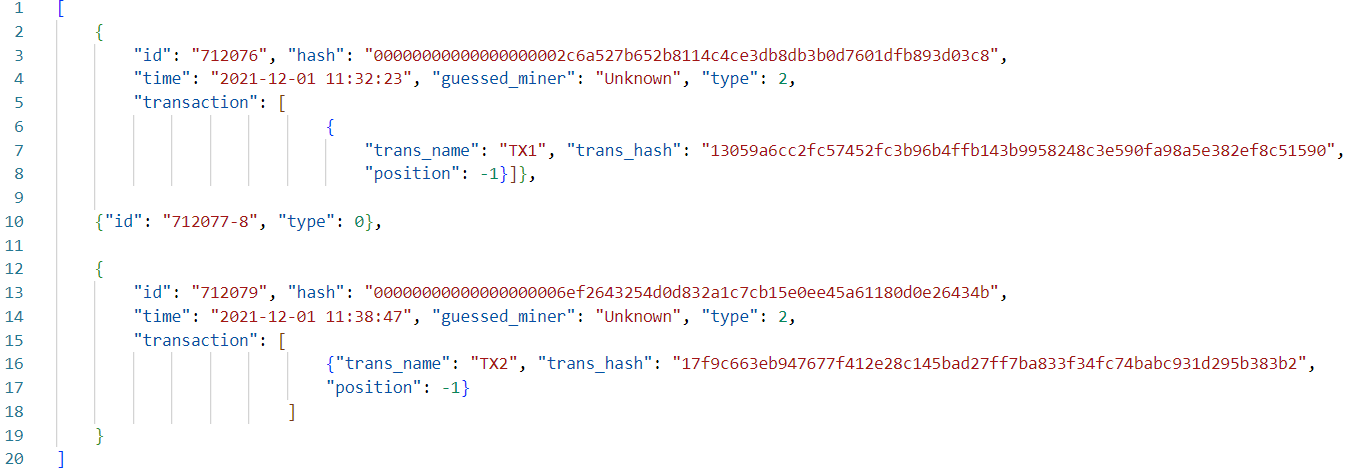
\includegraphics[keepaspectratio=true,scale=0.4]{Images/JSON_Definizione_TX.png}
    \caption{Struttura del JSON usato per il collegamento blocco-transazione}
\end{figure}

Per ogni blocco viene stilata una lista di transazioni validate al suo interno.
Nel caso in cui nella visualizzazione siano presenti dei blocchi, le cui transazioni non sono rilevanti, questi vengono semplificati tramite l'uso dei Cluster Block (riga 10).
BITVAS utilizza dei file ad hoc per le sue visualizzazioni.
Uno degli obiettivi cardine dell' API RESTful è la generazione dinamica di tali file partendo dai dati presenti all'interno del database a grafo.


\subsection{Architettura e diagramma di comunicazione}
Gli enormi vantaggi dell'architettura RESTful appurati in precedenza, la rendono la scelta migliore per lo sviluppo della API di questo progetto di tesi, la cui struttura e moduli sul quale si basa seguono il il seguente principio SRP.

\begin{center}
   \emph{``A module should be responsible to one, and only one, actor."} \cite{martin2018SoftwareStructure}
\end{center}
\thispagestyle{mystyle}
Il \emph{SRP (o Single-Responsibility-Principle)} \cite{PrinciplesOOD} \cite{martin2003agile} è uno dei principi fondamentali della programmazione orientata agli oggetti, il quale prevede che ogni modulo di un applicativo deve avere un solo motivo per essere modificato, ovvero una sola responsabilità , alla quale devono essere allineate tutte le funzionalità da essi offerte. Il motivo principale di tale principio è la diminuizione della complessità del progetto e il rischio di introdurre errori tramite la modifica del codice sorgente, aumentandone di conseguenza la scalabilità, la manutenibilità e la testabilità.
Per quanto concerne la programmazione di API, quanto detto si traduce nell'individuazione di endpoint specifici in grado di gestire dei task diversi e nella creazione di moduli completamente indipendenti l'uno dall'altro.

La struttura della API del progetto, infatti prevede quattro moduli separati, ognuno dei quali svolge un compito specifico: \emph{Index$\_$Server, JSON$\_$Controller, Query$\_$Controller, Request$\_$Controller}.

Index$\_$Server è il fulcro del middelware, pensato per occuparsi della gestione delle richieste da parte dei client e le corrispondenti risposte.
Con l'utilizzo delle tecnologie già citate permette al server di mettersi in ascolto di eventuali interrogazioni al database.

JSON$\_$Controller è un modulo utilizzato per la generazione dei file JSON strutturati in base ai dati richiesti.

Query$\_$Controller ha lo scopo di gestire e selezionare le varie query da inoltrare al server, a seconda delle necessità.

Request$\_$Controller è una classe utilizzabile dai client per poter integrare la API in altri applicativi.

\newpage
\thispagestyle{mystyle}
\begin{figure}[H]
    \centering 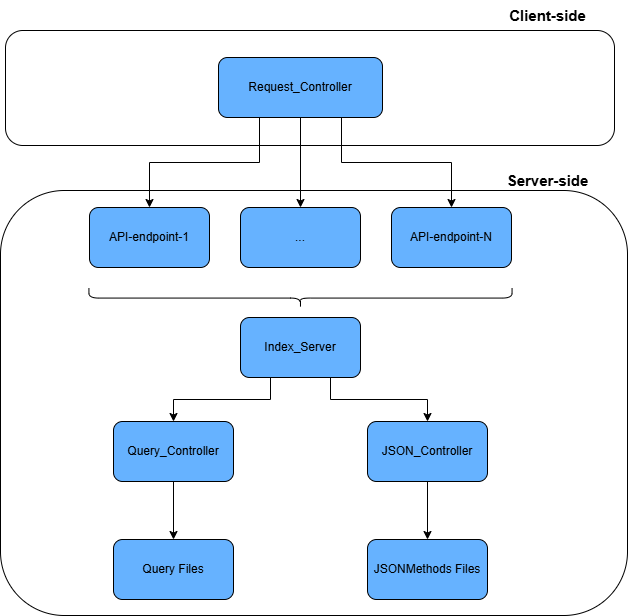
\includegraphics[keepaspectratio=true,scale=0.55]{Images/StrutturaInternaAPI.png}
    \caption{Struttura interna API}
\end{figure}

In figura 10 è mostrata la struttura interna della API, con tutti i moduli precedentemente elencati.
I due controller lato server, in base alle richieste, permettono di eseguire dei metodi finalizzati alla definizione delle query da inoltrare alla base di dati e quelli per la creazione dei JSON.
Tali metodi eseguono il codice sorgente di particolari moduli situati nelle cartelle \emph{Queries} e \emph{JSON methods}
L'indipendenza gli uni dagli altri di questi ultimi, permettono una gestione più semplice degli eventuali aggiornamenti futuri, legati allo sviluppo di nuove funzionalità.
Ad esempio se si volessero aggiungere altre visualizzazioni a BITVAS, si avrebbe la necessità di risucire ad estrapolare i dati necessari per generare le corrispettive risposte.
Per aggiornare il codice, basterebbe aggiungere i moduli per la query e la generazione dei file da inoltrare al client e modificare il codice dei controller, in modo da aggiungere dei metodi che permettano la gestione delle aggiunte effettuate.
Questa modularità fornisce maggior sicurezza in caso di modifica o aggiornamento del software, riducendo il rischio di errori.

\newpage
\thispagestyle{mystyle}
\begin{figure}[H]
    \centering 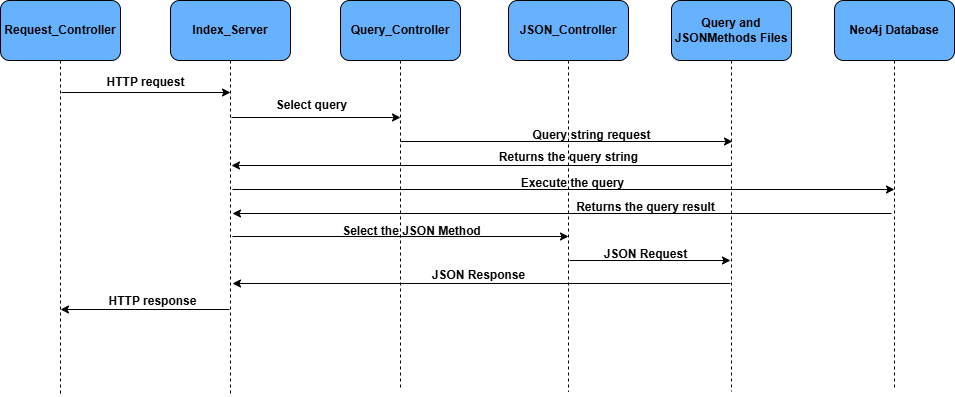
\includegraphics[keepaspectratio=true,scale=0.45]{Images/FlowChartAPI.png}
    \caption{Diagramma di sequenza della API}
\end{figure}

Attraverso il diagramma di sequenza mostrato in figura 11 è possibile individuare e comprendere nello specifico tutte le fasi della comunicazione tra i moduli dell'API RESTful sviluppata.

La prima fase consiste nell'inoltro da parte del client, tramite l'utilizzo di metodi specifici della classe Request$\_$Controller, di una richiesta HTTP verso il server.
Quest'ultimo, in attesa di interrogazioni, la gestisce come segue, tramite il file Index$\_$Server. A seconda dell'endpoint sollecitato e dei valori passati come parametri, attraverso l'utilizzo del modulo  Query$\_$Controller, viene estratta la query, sottoforma di stringa dal corrispondente file nella cartella Queries.
La stringa viene inviata al file Index$\_$Server, il quale la inoltra al database a grafo per poter estrapolare i dati necessari richiesti.
Il risultato delle query viene inoltrato al JSON$\_$Controller, tramite il quale si sceglie il metodo utile alla generazione dei file JSON,in grado di soddisfare le richieste del client, nella cartella JSONMethods.
Infine, questi ultimi vengono inviati al client, passando per la gesione di Index$\_$Server.

\subsection{Vantaggi architettura RESTful}

Presa in considerazione la natura dei due sistemi che si intende far interagire, l'architettura RESTful risulta la scelta più adeguata per lo sviluppo dell'API.
Quest'ultima infatti è molto efficace nel supporto di applicazioni web eseguite tramite browser, garantendo semplicità di utilizzo attraverso i metodi HTTP, ben conosciuti dagli sviluppatori. 

Inoltre grazie alla possibilità di utilizzare il protocollo HTTPS fornisce una maggiore sicurezza, proteggendo i dati durante il trasferimento.
Le informazioni possono essere trasferite dal server al client e viceversa attraverso molti formati di dati (JSON, XML, HTML, testo, ecc.), tutti indipendenti dalla piattaforma utilizzata, quindi interpretabili da ogni sistema operativo e da ogni dispositivo.

La leggerezza di questi formati combinata con la possibilià di memorizzare le risposte del server nella cache, garantisce un consumo minore della larghezza di banda rispetto ad altre soluzioni.

Infine grazie alla loro natura stateless e alla definizione di diversi endpoint per la gestione delle richieste, è possibile gestirne molte contemporaneamente.
La coesistenza di questi punti di forza permettono una gestione migliore del server, riducendone anche il carico computazionale, rendendo le API RESTful la scelta migliore per le web application.
\thispagestyle{mystyle}

\subsection{Endpoint}
Per garantire il Single-Responsibility-Principle di cui sopra, uno degli approcci fondamentali attuabili per quanto riguarda lo sviluppo di API è quello di identificare univocamente le risorse che possono essere richieste al server tramite la definizione di più endpoint, ognuno dei quali dedicato ad uno scopo specifico.
Più in dettaglio un endpoint è definibile come un URL  che funge da punto di interazione tra una API e un server, il quale si riferisce ad una singola risorsa.
I possibili parametri che è in grado di gestire si dividono in due tipi: \emph{in path} e  \emph{in query string}.
I parametri in path, utilizzati particolarmente per l'individuazione delle singole risorse, sono quelli che fanno parte dell'URL stesso.
Ad esempio, in \emph{https://urlexample.com/users/316704}, 316704 è un parametro nel percorso che potrebbe rappresentare l’ID di un utente.
Mentre quelli in query string, utili al filtraggio dei risultati di una richiesta, vengono aggiunti alla fine dell'URL dopo un 
punto interrogativo. Ad esempio, in  \emph{https://urlexample.com/search?q=books}, q=books è un parametro nella query string.

Tenendo conto della struttura dei dati necessari alla comunicazione del database di riferimento con \textit{BITVAS}, un endpoint che può essere definito riguarda l'estrapolazione delle informazioni per l'ottenimento delle visualizzazioni già sviluppate. L'identificazione di quest'ultimo avviene tramite l'URL \emph{http://localhost:7474/api/visualizations/:nomeVisual}.
 In questo caso si tratta di un endpoint che accetta richieste GET da parte dei client.
Uno dei parametri fondamentali è quello inserito nel percorso al posto di \emph{"nomeVisual"}, identificativo della visualizzazione che viene selezionata e della quale vengono prelevati i dati dal server, insieme al parametro \emph{"blockRef"} utile alla definizione del blocco centrale alle visualizzazioni progettate per \textit{BITVAS}.
Inoltre si può usufruire di un terzo parametro, ovvero \emph{"miner"}, necessario quando viene richiesta la MinerVisualization.

\newpage 
\begin{figure}[H]
    \centering 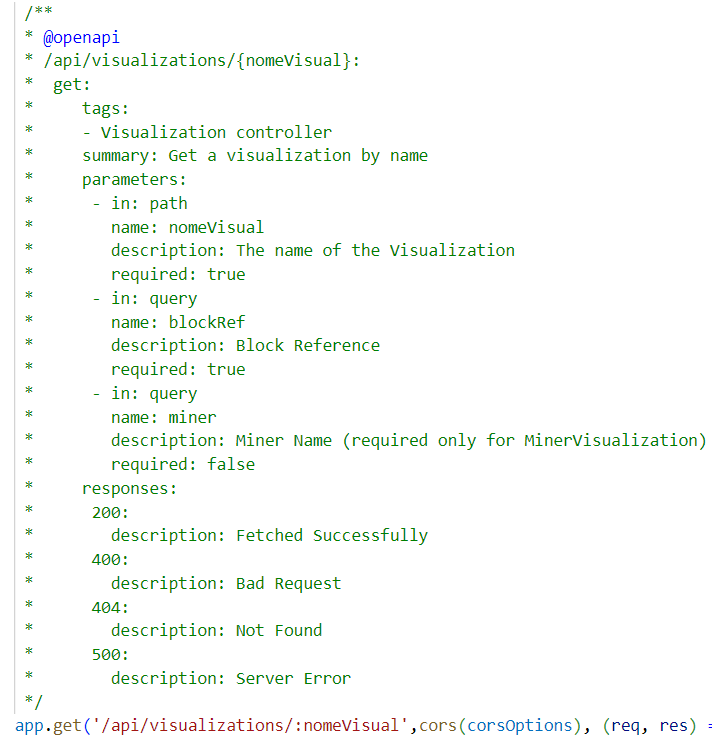
\includegraphics[keepaspectratio=true,scale=0.45]{Images/VisualizationEndpoint.png}
    \caption{Definizione endpoint tramite swagger UI e swagger-JSDocs}
\end{figure}

\thispagestyle{mystyle}

Oltre alla possibilità di estrazione dei dati necessari per il funzionamento del tool citato, L'\textit{API} mette a disposizione degli endpoint per permettere l'ottenimento di dati generici, utilizzabili in modi diversi a seconda delle esigenze.
Questi ultimi sono gestiti tramite l'URL  \\
\emph{http://localhost:7474/api/entities/:entityName}, il quale permette di ottenere i dettagli sulle entità presenti all'interno della base di dati.
Il parametro nel percorso \emph{"entityName"} identifica il tipo di entità, come transazioni, blocchi o i cluster progettati (hour, day, month e year). La selezione vera e propria di essa avviene con il timestamp attaverso il primo parametro in query string, ovvero \emph{"startTimestamp"}.
Se viene usato anche il parametro \emph{"endTimestamp"}, vengono estratti i dati di un insieme di entità, i cui timestamp sono compresi in un range temporale definito da entrambi i parametri.

Uno dei vantaggi dell'utilizzo dei database a grafo è quello di evidenziare le relazioni tra i dati presenti al suo interno, che in questo caso specifico pongono l'attenzione sui flussi di Bitcoin.
Per poter prelevare tali dati si può effettuare una richiesta all'URL 
 \\
 \emph{http://localhost:7474/api/flows/:ClusterToCluster}, dove \emph{"ClusterToCluster"} individua le entità coinvolte nel flusso da estrarre (es. DayToDay o BlockToYear). Con i parametri in query string \emph{"Timestamp"} e \emph{"RangeTimestamp"} si selezionano rispettivamente, il punto di arrivo e il range di partenza del flusso di Bitcoin.
Ad esempio utilizzando \textit{'2024-01-05'} e \textit{'2023-12-07T04,2023-12-07T09'}, vengono estrapolati i flussi uscenti dagli hour-cluster appartenenti al range definito che arrivano al day-cluster selezionato.

\subsection{Funzionalità progettate}
Le funzionalità progettate per la API riguardano nello specifico le tre categorie in linea con gli endpoint esposti.
Le prime utili all'interazione del database a grafo e BITVAS sono le seguenti:

\begin{itemize}
    \item \emph{getBlockVisualizationFirstPart(blockRef)} : Preso in input un riferimento al blocco, più precisamente un timestamp, restituisce la prima parte della BlockVisualization composta dai flussi di Bitcoin che partono da blocchi con timestamp ad una distanza temporale di massimo dodici ore e arrivano al blocco selezionato.

    \item \emph{getBlockVisualizationSecondPart(blockRef)} : Preso in input un riferimento al blocco, più precisamente un timestamp, restituisce la seconda parte della BlockVisualization composta dai flussi di Bitcoin partono dal blocco selezionato e arrivano ai blocchi con timestamp ad una distanza temporale di massimo dodici ore.

    \item 
    \emph{getCombinedVisualization(blockRef)}: Preso come parametro il timestamp identificativo del blocco centrale alla visualizzazione, restituire tutti i blocchi compresi nelle dodici ore precedenti e successive ad esso con tutte le relative relazioni, rappresentative dei flussi di Bitcoin. In questo caso i flussi fanno riferimento a tutti i blocchi compresi nell'arco temporale giornaliero.
\thispagestyle{mystyle}
    \item 
    \emph{getTXVisualizationFirstPart(hash)}: Preso in input un hash identificativo di una transazione, vengono restituite tutte le relazioni rappresentanti i flussi di Bitcoin in uscita ad essa.

    \item 
    \emph{getTXVisualizationSecondPart(hash)}: Preso in input un hash identificativo di una transazione, vengono restituite tutte le relazioni rappresentanti i flussi di Bitcoin in ingresso ad essa.
    
    \item 
    \emph{getMinerVisualizazion(blockRef, miner)}: Preso in input un timestamp identificativo del blocco centrale della visualizzazione e un miner specifico (es. Binance), restituisce tutti i flussi di Bitcoin riguardanti i blocchi compresi nelle dodici ore precedenti e successive al blocco scelto e che sono stati minati dallo stesso miner.
\end{itemize}

Per alcune visualizzazioni, come la BlockVisualization e la TXVisualization si è optato per la separazione in due funzioni distinte, per garantire un utilizzo più generale dei dati.
Infatti, questo è stato possibile soprattutto considerando la presenza nella loro struttura di un blocco sul quale viene concentrata l'attenzione per la rappresentazione dei flussi.
Questi ultimi, nei due casi sopra citati si dividono in due tipi, ovvero quelli che partono dal riferimento selezionato, e quelli che arrivano a tale elemento.

Come già trattato in precedenza, per permettere l'integrazione del database con altri applicativi in grado di porre il focus sui flussi temporali di Bitcoin.

\begin{figure}[H]
    \centering 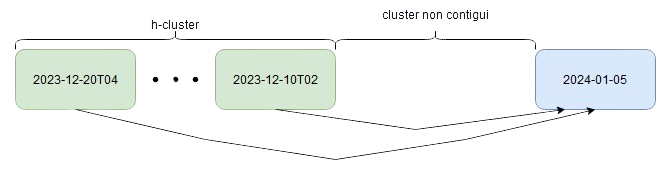
\includegraphics[keepaspectratio=true,scale=0.6]{Images/FlowsExampleQuery.png}
    \caption{Esempio di flusso tra hour cluster e day cluster}
\end{figure}

La rappresentazione può prevedere l'interazione tra cluster di tipo di verso che possono essere contigui e non. Per L'API sviluppata sono state definite le seguenti funzionalità:
\thispagestyle{mystyle}
\begin{itemize}

    \item \emph{getBlockToDayFlows(dClusterDate,BlocksTimestampRange)} : il primo parametro identifica il day cluster da prendere in considerazione (es. 2024-01-05), mentre il secondo sta ad indicare un insieme di blocchi, i cui timestamp sono compresi nel range \\ (es. 2024-01-05T03:56:00Z,2024-01-05T05:56:00Z).
    La funzione restituisce tutti i flussi di Bitcoin che partono dal range indicato e hanno come punto di arrivo il cluster selezionato.
    
    \item \emph{getHourToDayFlows(dClusterDate,hClusterRange)}:
    Preso in input un parametro identificativo di un day-cluster (es. 2024-01-05) e un range di timestamp che indicano un insieme di hour-cluster (es.  2024-01-05T03,2024-01-05T05), restituisce tutti i flussi di cryptovaluta che partono da questi ultimi e arrivano al day-cluster selezionato.
    
    \item \emph{getDayToDayFlows(dClusterDate,dClusterRange)} : in questo caso, vengono restituiti i flussi che partono e arrivano a cluster diversi della stessa tipologia. 
    \textit{dClusterDate} indica l'entità di arrivo dei flussi, mentre \textit{dClusterRange} rappresenta l'insieme dei cluster di partenza.

    
    \item \emph{getMonthToDayFlows(dClusterDate,mClusterRange)} : \emph{dClusterDate} individua il cluster di arrivo dei flussi di Bitcoin, mentre \emph{mClusterRange} indica un insieme di entità rappresentative dei mesi dai quali partono.
    
    \item \emph{getYearToDayFlows(dClusterDate,yClusterRange)} : restituisce i flussi di Bitcoin che partono dagli year-cluster, identificati tramite il parametro \emph{yClusterRange} (es. 2023,2024) e arrivano al dCluster selezionato tramite il primo parametro.
\end{itemize}

In questo caso vengono presi in considerazione i flussi di Bitcoin in entrata ai day-cluster, la cui struttura può essere ripetuta anche per gli altri cluster.

Oltre al focus ai suddetti flussi, l'API permette di poter estrarre dati generici riguardanti i dettagli delle entità presenti all'interno del database. Le funzioni sviluppate per tale scopo sono le seguenti : 

\begin{itemize}
    \item \emph{getTXInfo(startTimestamp,endTimestamp)} : restituisce le informazioni legate alle transazioni, il cui timestamp definito dal primo parametro.
    Il secondo parametro, ovvero \emph{endTimestamp} è opzionale e viene utilizzato nel caso in cui si vogliano conoscere i dati di transazioni comprese in un range di timestamp.

    \item \emph{getBlockInfo(startTimestamp,endTimestamp)} :
    restituisce i dettagli di un blocco nel caso in cui sia inizializzato solo il parametro \emph{startTimestamp}.
    Se viene definito anche il secondo parametro, vengono restituite tutte le informazione dei blocchi i cui timestamp sono compresi nell'intervallo temporale indicato dai due parametri.
    \item \emph{getXClusterInfo(startXTime,endXTime)} : è una generalizzazione delle funzioni programmate per il reperimento dei dettagli legati ai vari cluster nel database (es. \emph{getHClusterInfo} per gli hour-cluster)..
    Come per quelle precedenti, l'inizializzazione del solo primo parametro  permette di restituire i dati dei cluster identificati da esso.
    Nel caso in cui venga definito anche \emph{endXTime} vengono restituite le informazioni dei cluster appartenenti all'arco temporale indicato dai due parametri.
\end{itemize}
\thispagestyle{mystyle}
Tali funzioni sono strutturati in moduli separati e indipendenti tra loro, in modo da facilitare la manutenzione e l'aggiornamento del sistema, garantendo una maggiore scalabilità ed adattabilità a seconda delle esigenze.


\subsection{Moduli API}
In questa sezione vengono analizzati nel dettaglio i vari moduli dell'API sviluppata.
Le API sono componenti essenziali che permettono la comunicazione tra diversi applicativi, facilitando l'accesso e la manipolazione dei dati in modo efficiente e sicuro.
L'architettura modulare della API presentata in questa tesi è stata progettata con lo scopo di garantire scalabilità, manutenibilità e adattabilità del sistema.
Ogni modulo è stato sviluppato in modo da essere indipendente dagli altri con l'obiettivo di svolgere dei compiti specifici, riducendo la complessità di comprensione e modifica del codice sorgente.

\subsubsection{Index$\_$Server}
Index$\_$Server è il modulo principale dell'API, tramite il quale il server si mette in ascolto, su una determinata porta, in attesa di eventuali richieste da parte di possibili client.
Attraverso l'utilizzo di particolari moduli vengono definiti i parametri necessari alla connessione, tra cui anche le opzioni per a gestione del \emph{CORS(Cross-Origin Resource Sharing)}.

Il CORS \cite{CORS} è un meccanismo di sicurezza messo in atto dai browser in grado di permettere ai server di effettuare un controllo sulle risorse che possono essere richieste da un dominio diverso da quello in cui il server stesso è caricato.
La sua gestione risulta molto utile quando si ha a che fare con API il cui scopo è quello di accedere a risorse esterne come i database.
Inolte previene possibili attacchi malevoli nei quali un sito esterno potrebbe inviare richieste non autorizzate usando le credenziali degli utenti.


\begin{figure}[H]
    \centering 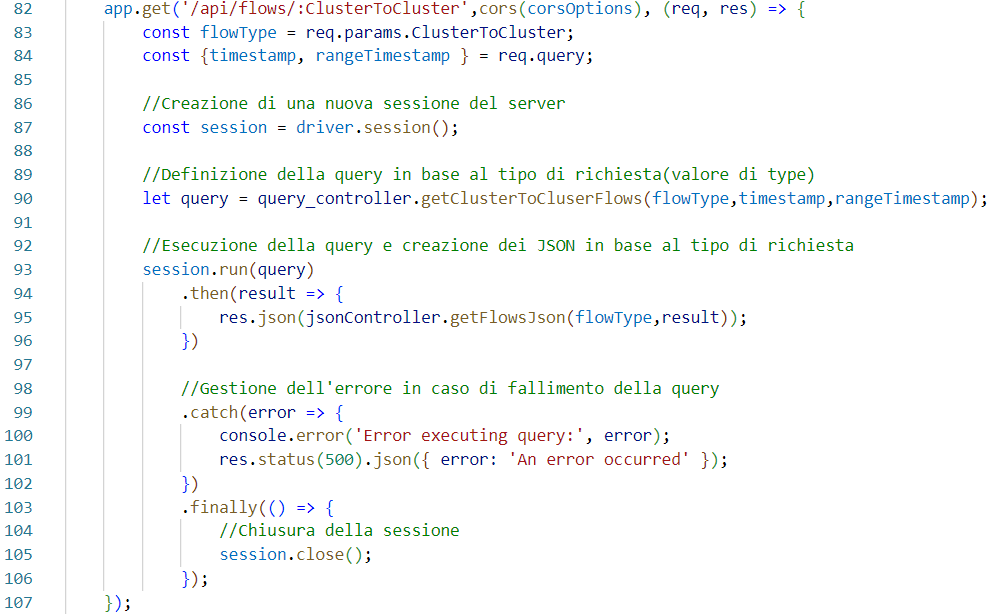
\includegraphics[keepaspectratio=true,scale=0.5]{Images/Index_Server_Endpoint.png}
    \caption{Definizione endpoint e gestione delle richieste}
\end{figure}

In figura 14 viene mostrato il codice sorgente riguardante l'inizializzazione di un endpoint, finalizzata tramite un'istanza del framework Express (riga 82), con i cui metodi è possibile definire il tipo di richieste che possono essere accettate (get,post,put,delete). Oltre alla scelta dell'URL identificativo dell'endpoint attraverso il quale si possono inoltrare richieste anche tramite browser, possono essere utilizzati altri parametri per ampliarne la gestione, come le opzioni per gestire il meccanismo CORS.

\thispagestyle{mystyle}
La gestione delle richieste avviene per fasi distinte.
In primis viene definita una sessione, tramite un'istanza dei driver di collegamento di neo4j, con il database a grafo sviluppato.
A seconda dell'endpoint a cui si fa riferimento, viene estrapolata la query da inoltrare tramite l'apposito controller, che successivamente viene inoltrata alla base di dati con l'istanza della connessione (riga 93).
Il risultato, gestito in modo asincrono, viene infine utilizzato per la creazione della risposta da inviare ai client, tramite il controller usato per la creazione dei JSON, previo eventuale controllo su possibili errori che possono verificarsi durante l'esecuzione. Al termine della gestione della richiesta la sessione al database viene chiusa.

Particolarmente importante è anche la gestione del caching, attuata con il modulo \emph{apicache} intallabile tramite npm, per permettere al server di gestire richieste ridondanti da parte del client, nell'arco di cinque minuti, in maniera tale da diminuire il carico sul server e velocizzare il reperimento dei dati lato client.

\subsubsection{Json$\_$Controller}
Il modulo JSON$\_$Controller è quello che si occupa di gestire la logica che intercorre tra il flusso di dati proveniente dal database e il client che ne richiede le informazioni, in modo da assolvere alla necessità di chiarezza nei dati e semplicità della struttura del sistema sviluppato garantendo tutti i principi precedentemente citati.
Si può considerare come il modulo centrale tramite il quale vengono effettuate delle scelte relative ai file JSON da generare, a seconda dei parametri utilizzati per la richiesta dei dati.
\thispagestyle{mystyle}
\begin{figure}[H]
    \centering 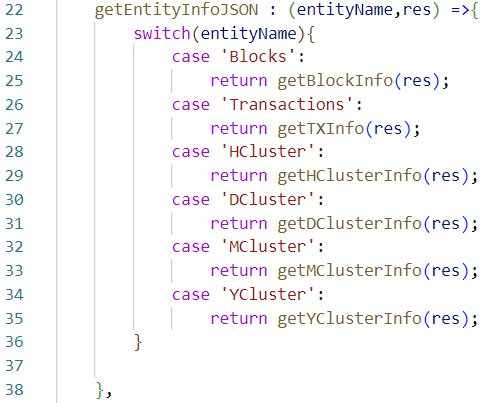
\includegraphics[keepaspectratio=true,scale=0.5]{Images/JSONControllerMethod.png}
    \caption{metodo JSON$\_$Controller per la scelta delle risposte da generare}
\end{figure}

In figura 15 è mostrata la scelta della struttura del file da inoltrare al client, in base alla richiesta ricevuta, legato alle informazioni delle entità presenti nella base di dati.
In questo caso a seconda del tipo di entità di cui si vogliono estrarre gli attributi, viene richiamato il modulo corrispondente al JSON da generare, nella cartella JSON Methods.

\subsubsection{Query$\_$Controller}
Il modulo Query$\_$Controller viene utilizzato come intermediario nella comunicazione tra il server e la cartella Queries contenente i file utilizzabili per l'estrapolazione delle query da inoltrare al database.
Come mostrato in figura 16, in base alla richiesta del client, distinguibile dai parametri inizializzati, viene estratta una query diversa, tramite i moduli importati.

\begin{figure}[H]
    \centering 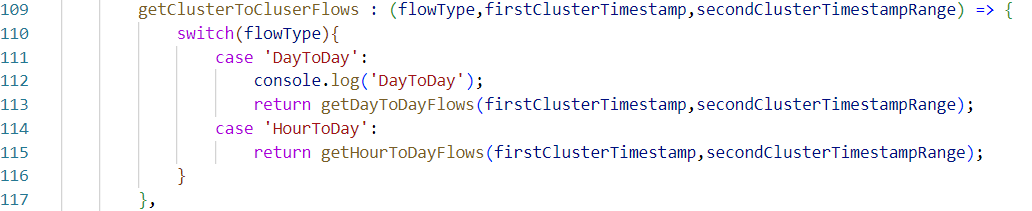
\includegraphics[keepaspectratio=true,scale=0.5]{Images/ExampleQueryControllerMethod.png}
    \caption{metodo Query$\_$Controller per l'estrazione delle query da inoltrare al database}
\end{figure}
\thispagestyle{mystyle}
Nel caso specifico mostrato, a seconda del tipo di entità coinvolte nel flusso richiesto viene estratta la Cypher query corrispondente. 

Per garantirne la corretta estrapolazione tramite l'utilizzo del modulo Request$\_$Controller, si occupa anche di individuare i tipi dei cluster coinvolti nei flussi, tramite l'apposito metodo getClusterType().
Quest'ultimo accetta come parametri in ingresso i timestamp dei cluster dei flussi che si vogliono estrarre, e restituisce il loro tipo 
(es. DClusterTimestamp se il timestamp è di un d-cluster), tramite i quali si hanno tutte le informazioni necessarie per definire la query string da inviare al server.
\subsubsection{JSONMethods Files e Query Files}

Per garantire scalabilità e manutenibilità del codice in linea con il principio SRP, si è deciso di sviluppare moduli indipendenti per l'estrapolazione delle query da inoltrare al database e per la generazione dei JSON, in modo che possano essere richiamati all'occorrenza dagli appositi controller.
In questo modo si facilita anche la comprensione del codice sorgente e si rende più semplice l'aggiunta di nuove funzionalità.
I file rappresentativi dei moduli si trovano nelle cartelle Queries e JSON Meethods e vengono importati nei moduli controller già trattati in precedenza.

\begin{figure}[H]
    \centering 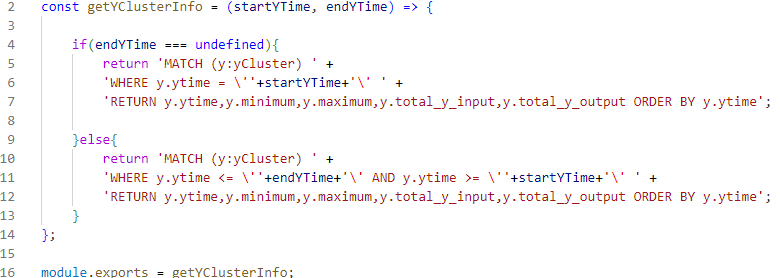
\includegraphics[keepaspectratio=true,scale=0.7]{Images/esempioModuliQuery.png}
    \caption{modulo per l'ottenimento della query getYClusterInfo()}
\end{figure}

\begin{figure}[H]
    \centering 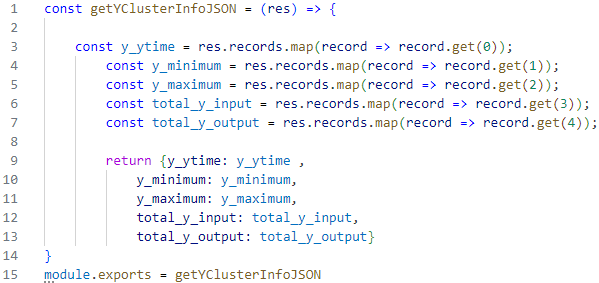
\includegraphics[keepaspectratio=true,scale=0.7]{Images/esempioModuliCreazioneJSON.png}
    \caption{modulo generazione JSON per la query getYClusterInfo()}
\end{figure}
\thispagestyle{mystyle}

\begin{onehalfspacing}
\subsubsection{Request$\_$Controller}
Il modulo Request$\_$Controller è di fondamentale importanza per garantire la comunicazione tra client e server, fungendo da interfaccia al database messo a disposizione.
Più nel dettaglio è una classe scritta in Javascript il cui unico attributo è un'istanza della classe XMLHttpRequest, che viene utilizzato per inoltrare le richieste HTTP al server, la cui query string viene definita a seconda del metodo richiamato e dai parametri utilizzati.

\thispagestyle{mystyle}

\begin{figure}[H]
    \centering 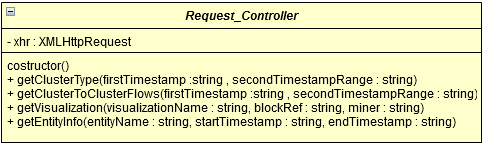
\includegraphics[keepaspectratio=true,scale=1]{Images/UMLRequestController.png}
    \caption{Diagramma UML della classe Request$\_$Controller}
\end{figure}

Quando viene richiamato il metodo per l'ottenimento dei flussi tra cluster, per identificarne il tipo viene fatto uso del metodo getClusterType, il quale prende come parametri i timestamp dei cluster e restituisce il loro tipo (es. una stringa contenente BlockTimestamp oppure HClusterTimestamp).
\end{onehalfspacing}

  
\end{onehalfspacing}

\clearpage
\section{Test e validazione \textit{API}}
\begin{onehalfspacing}
  In questo capitolo vengono descritti gli strumenti e la metodologia adottati per la fase di test dell'API sviluppata. L'obiettivo è quello di garantire il corretto funzionamento di quest'ultima nel reperimento dei presenti nel database a grafo, tramite la documentazione messa a punto tramite Swagger.



\subsection{Test tramite Swagger Documentation}
Come già trattato in precedenza attraverso alcuni moduli di Swagger è possibile definire una documentazione interattiva, intuitiva e semplice da utilizzare al fine di testare gli endpoint dell'API sviluppata.
I due moduli necessari alla sua definizione sono swagger-ui-express e swagger-jsdoc, installati tramite npm e integrati nel codice sorgente del modulo Index$\_$Server.
L'interazione avviene tramite browser, consentendo di eseguire richieste e visualizzare risposte in tempo reale, tramite l'endpoint \emph{http://localhost:7474/api-docs}.

Ogni endpoint deve essere commentato come già spiegato in precedenza, per poter essere inserito e testato nella documentazione. Di seguito vengono mostrati i test effettuati per ognuno di essi.


\begin{figure}[H]
    \centering 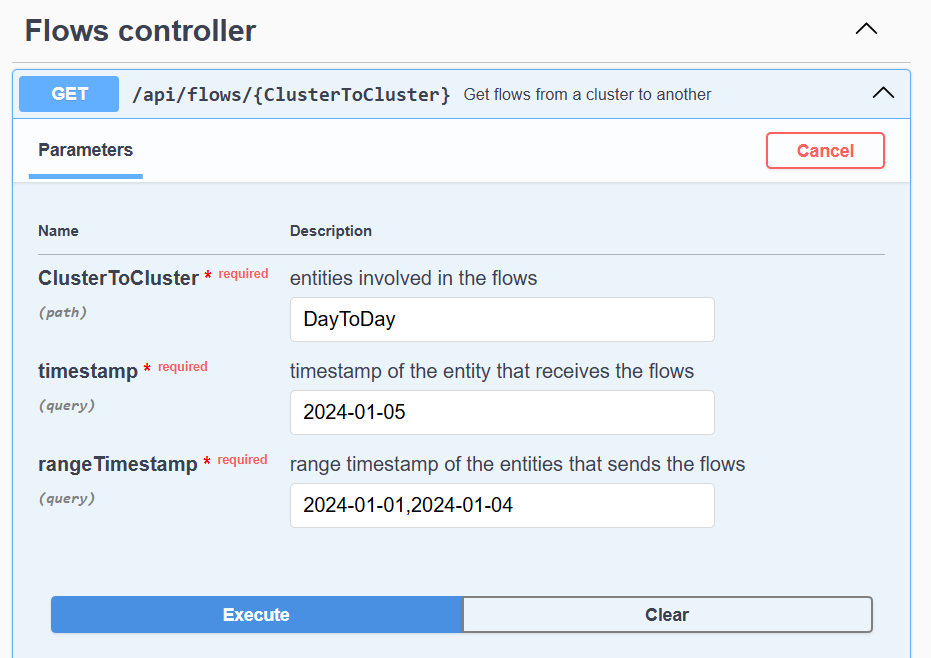
\includegraphics[keepaspectratio=true,scale=0.5]{Images/FlowControllerTestSwagger.png}
    \caption{Schermata Flow Controller della documentazione}
\end{figure}

In questo caso vengono richiesti i flussi tra Day-Cluster, il cui punto di partenza è definito dalle entità il cui timestamp è compreso nell'arco temporale che va dal 2024-01-01 al giorno 2024-01-04, mentre il punto di arrivo è il cluster con timestamp 2024-01-05.

\begin{figure}[H]
    \centering 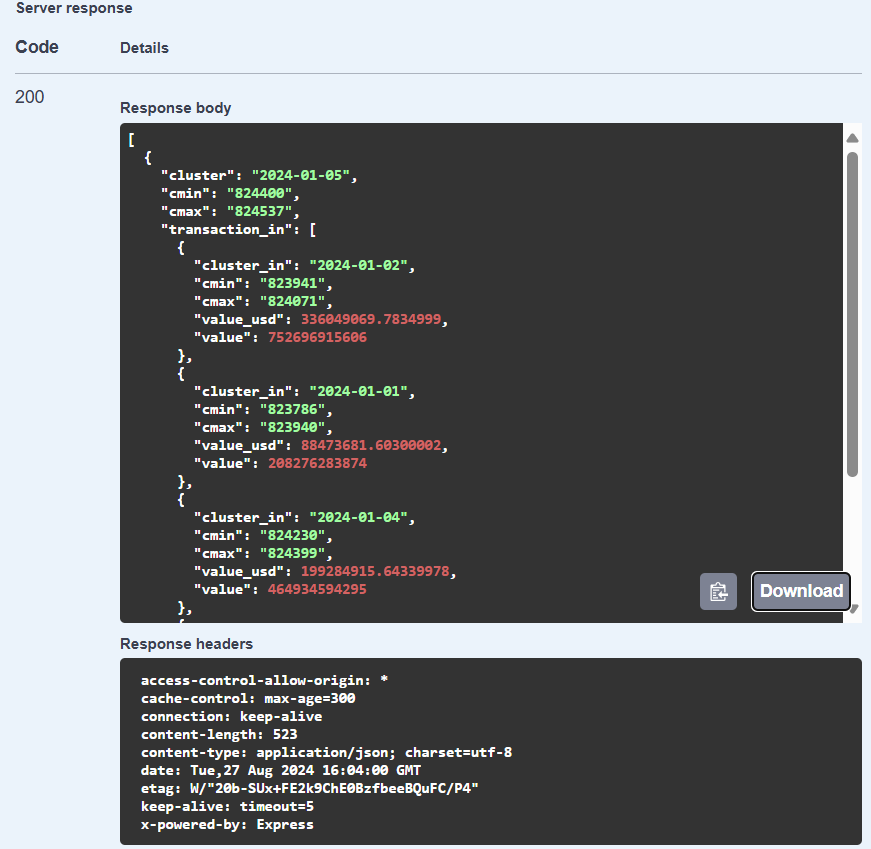
\includegraphics[keepaspectratio=true,scale=0.5]{Images/responseFlowController.png}
    \caption{Risposta della query effettuata tramite Flow Controller}
\end{figure}
In figura 21 viene mostrata la risposta inoltrata dal server per la gestione della richiesta effettuata tramite la sezione Flow Controller della documentazione.
La struttura generata per il JSON è in linea con quelle utilizzate per le visualizzazioni di BITVAS.
Ogni elemento dell'array corrisponde ai cluster di arrivo dei flussi considerati, che in questo caso è solo quello definito dal parametro timestamp, ovvero 2024-01-05.
L'array transaction$\_$in viene utilizzato per interpretare e rappresentare i flussi, infatti al suo interno vengono immagazzinati i Day-Cluster di partenza di questi ultimi, con relativo volume di cryptovaluta speso. 
\thispagestyle{mystyle}
\begin{figure}[H]
    \centering 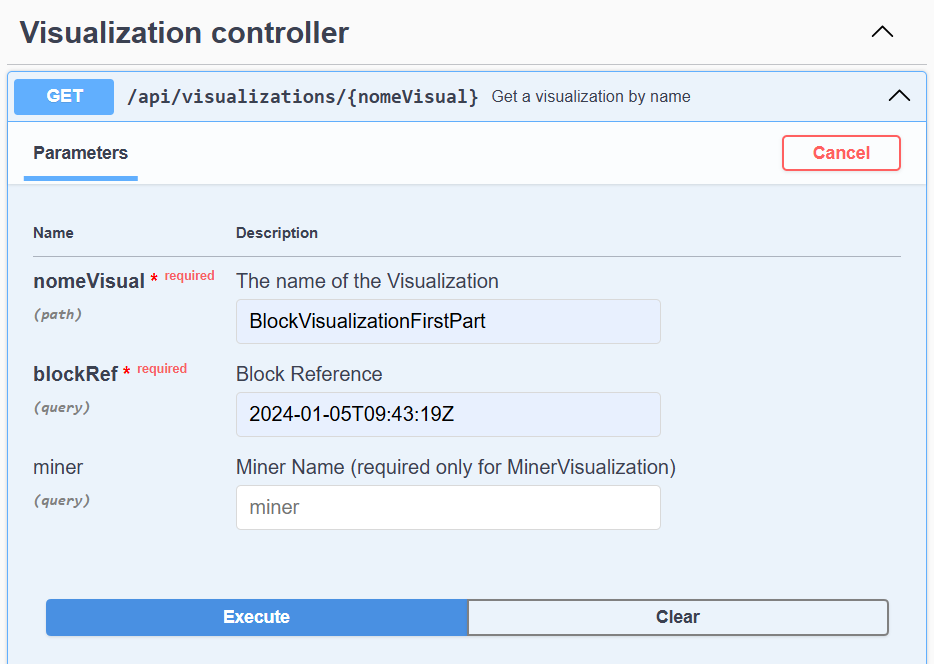
\includegraphics[keepaspectratio=true,scale=0.5]{Images/VisControllerSwaggerTest.png}
    \caption{Schermata Visualization Controller della documentazione}
\end{figure}
In questo caso, i parametri inseriti in input riguardano il nome della visualizzazione che si vuole ottenere, ovvero la prima parte della BlockVisualization e il timestamp di riferimento del blocco centrale di essa.
I risultati ottenuti e visualizzati di seguito, seguono la struttura dei file JSON già trattati in precedenza.
Per l'elemento che rappresenta il blocco centrale viene inizializzato un array, al cui interno vengono inseriti gli attributi riguardanti i blocchi da cui partono i flussi di Bitcoin.

La risposta fornita dal server fornisce solamente la prima parte della BlockVisualization, la quale si focalizza sui flussi in ingresso al blocco centrale.
Unendo quest'ultima con la risposta derivata dalla richiesta della seconda parte, si ottiene la risposta completa da integrare con BITVAS.

La scelta di effettuare una divisione della richiesta è dovuta alla possibilità di riutilizzo di tali dati in maniera diversa da quella definita dal tool di visualizzazione preso in esame.Questo approccio modulare consente una maggiore flessibilità nell’analisi dei dati, permettendo di eseguire query specifiche e di ottenere risposte mirate per diverse esigenze analitiche. Inoltre, facilita l’aggiornamento e la manutenzione del sistema, poiché ogni parte della visualizzazione può essere gestita e ottimizzata separatamente.
\thispagestyle{mystyle}
\begin{figure}[H]
    \centering 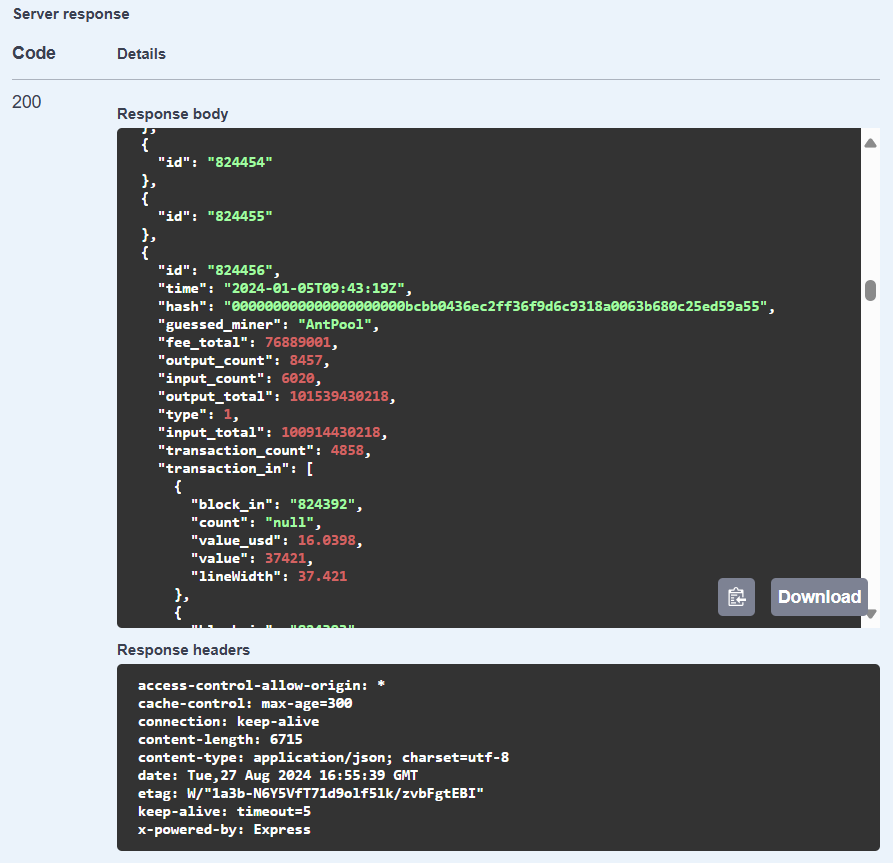
\includegraphics[keepaspectratio=true,scale=0.45]{Images/responseVisController.png}
    \caption{Risposta della query effettuata tramite Flow Controller}
\end{figure}


\begin{figure}[H]
    \centering 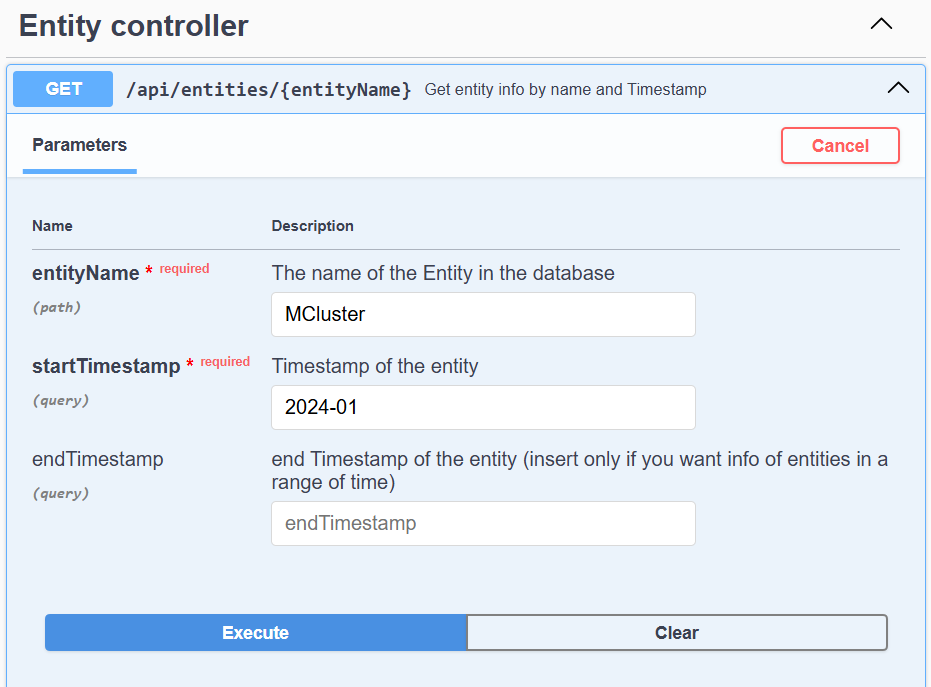
\includegraphics[keepaspectratio=true,scale=0.4]{Images/EntityControllerSwaggerTest.png}
    \caption{Schermata Entity Controller della documentazione}
    
    \thispagestyle{mystyle}
\end{figure}

In figura 24 viene mostrata la richiesta per le informazioni riguardanti un determinato Month-Cluster, identificato dal timestamp 2024-01.
\begin{figure}[H]
    \centering 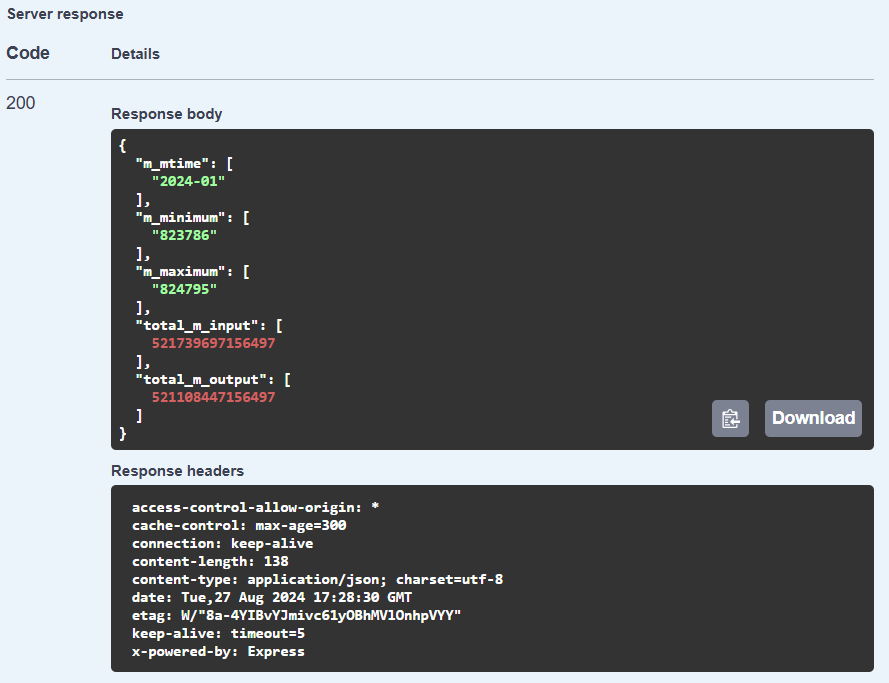
\includegraphics[keepaspectratio=true,scale=0.6]{Images/responseEntityController.png}
    \caption{Risposta della query effettuata tramite Entity Controller}
\end{figure}

La risposta fornita dal server è un file JSON i cui elementi sono degli array, ognuno dei quali corrisponde ad un attributo delle entità esratte, tra cui anche l'id minimo e massimo dei blocchi a cui essa fa riferimento.
In questo caso sono state richieste le informazioni di un solo MCluster, quindi è presente un solo elemento per ogni attributo.
\thispagestyle{mystyle}
Inoltre come per le risposte visualizzate precedentemente insieme alla risposta viene restituito un header con alcuni parametri fondamentali tra cui quelli utilizzati per la gestione del caching o il tipo contenuto in essa.

\subsection{Test di integrazione con BITVAS}
In questa sezione vengono mostrati i test effettuati per verificare il corretto reperimento dei dati necessari alle visualizzazioni di BITVAS.

L'API strutturata permette l'utilizzo del database a grafo ad applicativi esterni tramite la classe Request$\_$Controller, che mette a disposizione dei metodi per effettuare delle richieste GET al server.
Quest'ultima è stata integrata nel codice sorgente di BITVAS, in modo tale da rendere dinamico il reperimento dei dati.


\begin{figure}[H]
    \centering 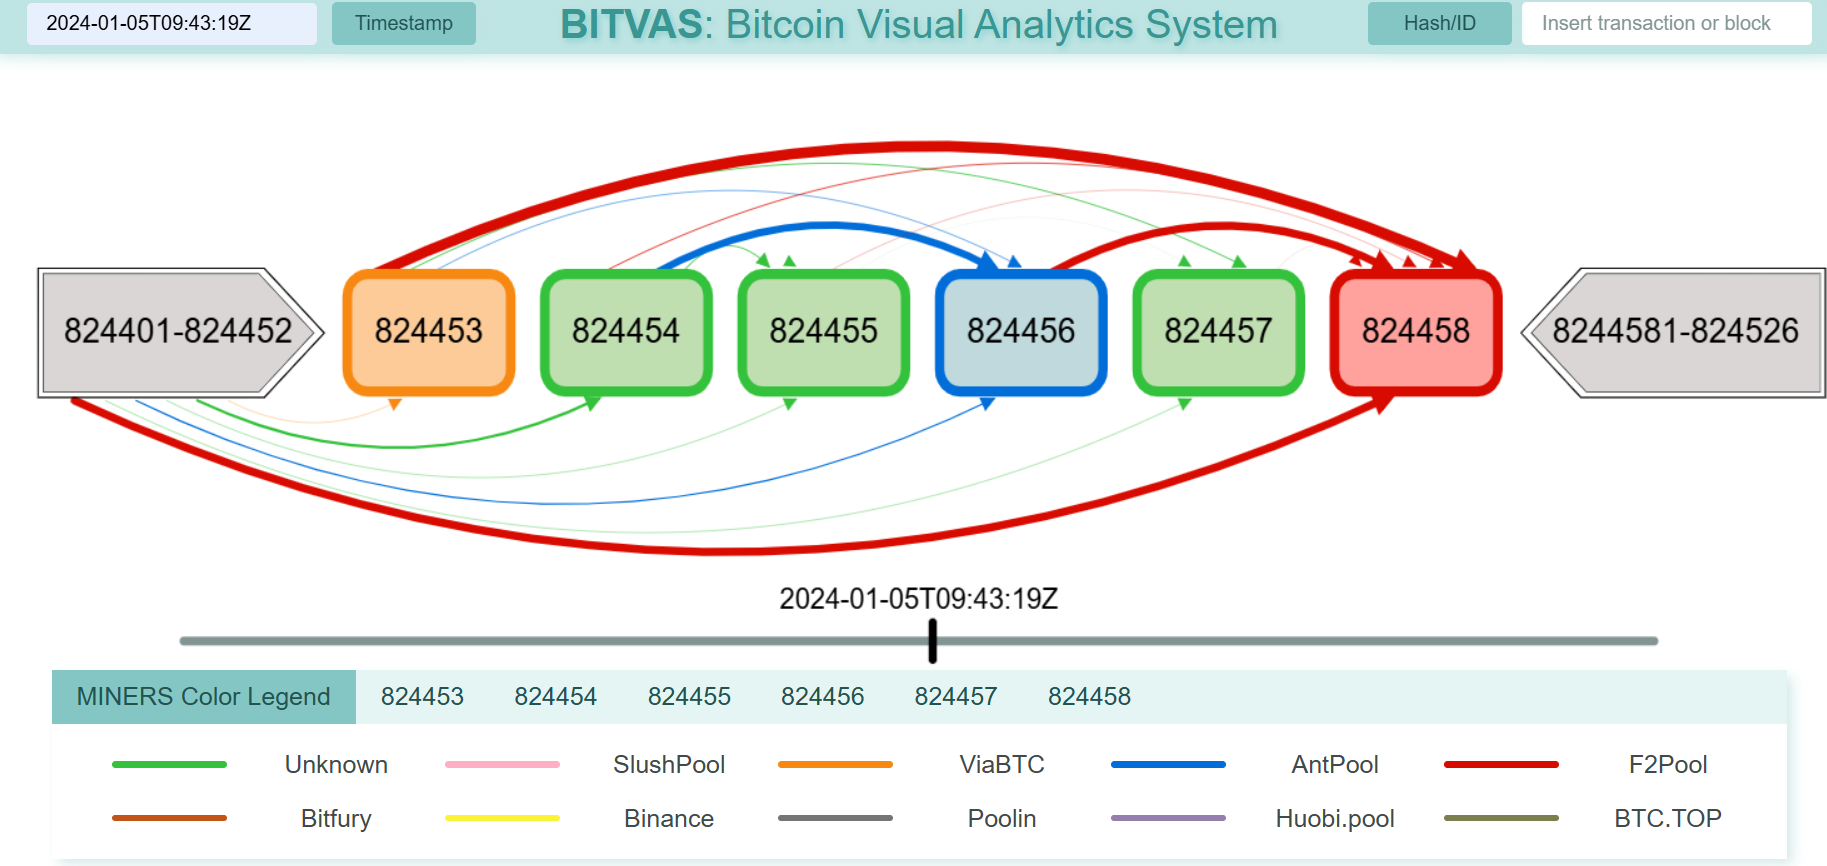
\includegraphics[keepaspectratio=true,scale=0.3]{Images/CombinedVisTested.png}
    \caption{Test CombinedVisualization}
\end{figure}

In figura 26 viene mostrata la visualizzazione dopo l'inserimento del timestamp '2024-01-05T09:43:19Z' in alto a sinistra, il cui blocco identificato da esso viene generato al centro della visualizzazione (824456).
Quest'ultimo si può modificare con lo slider posto al di sotto dei blocchi, traslando la visualizzazione blocco per blocco. 
Come ultimo elemento della schermata è presente una legenda interattiva con la quale richiedere la minerVisualization.
Nel caso del test effetuato viene scelto il miner 'AntPool', la cui visualizzazione viene mostrata di seguito.

\begin{figure}[H]
        \centering 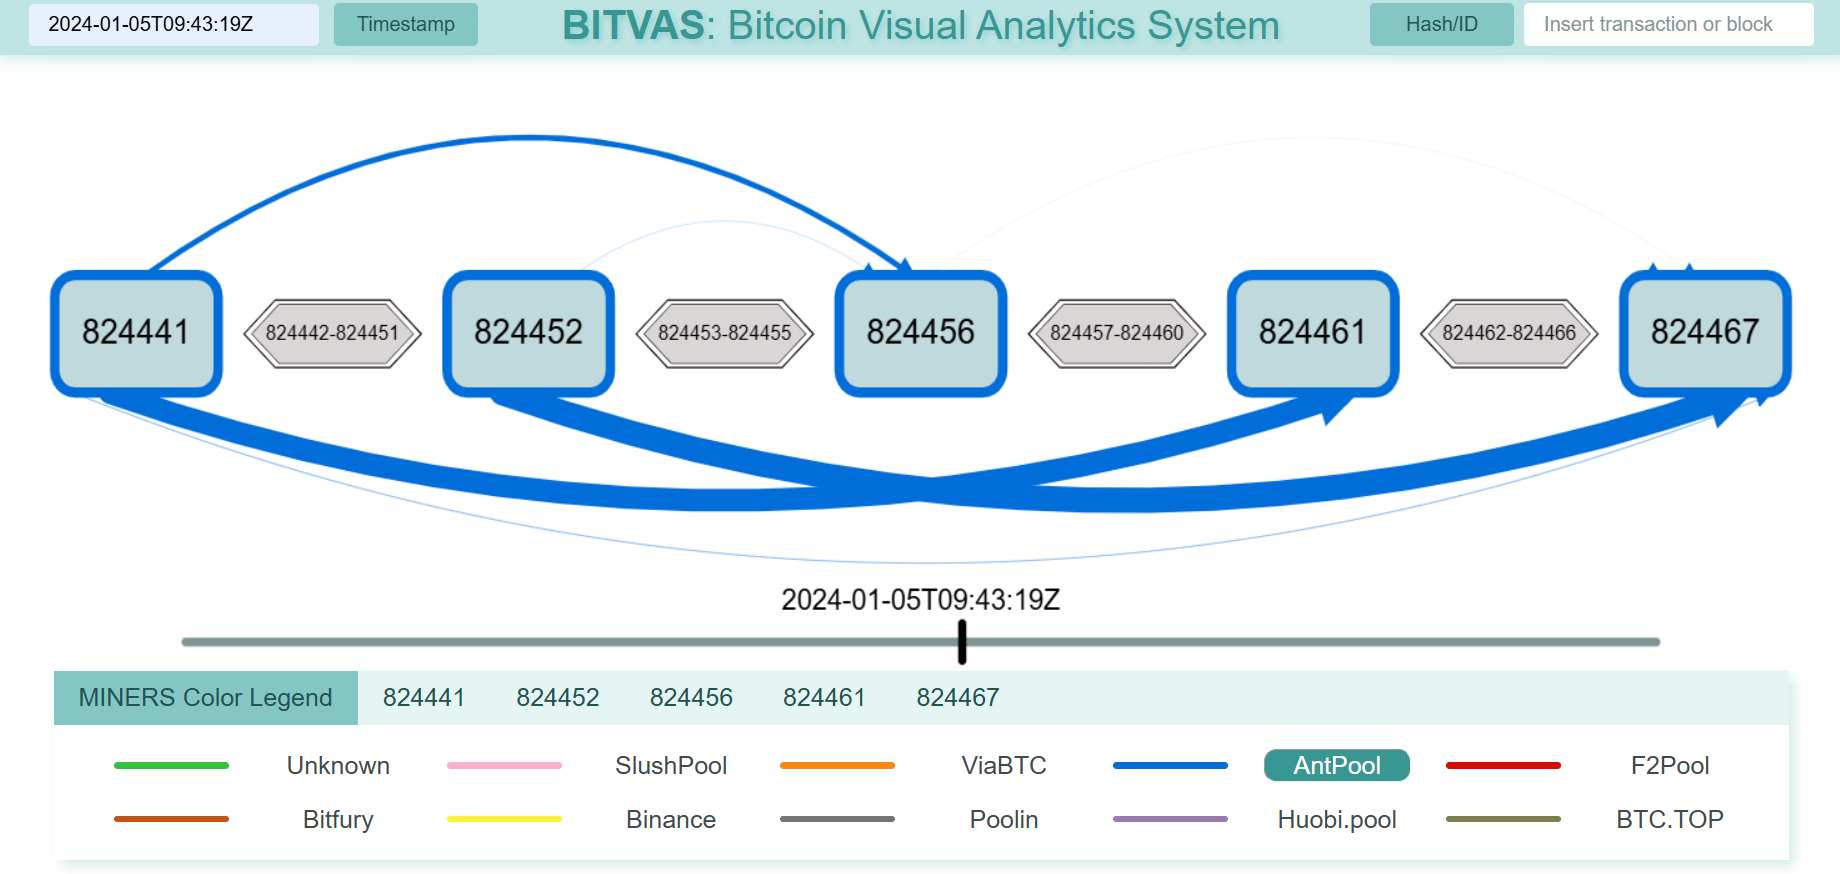
\includegraphics[keepaspectratio=true,scale=0.28]{Images/MinerVisualizationTest.png}
    \caption{Test MinerVisualization}
\end{figure}
\thispagestyle{mystyle}
Anche in questo caso il blocco identificato dalla posizione dello slider, ovvero quello inserito come input per la visualizzazione iniziale, si trova al centro di essa.
Nel caso in cui il blocco scelto non faccia parte dei flussi legati al miner selezionato, tramite i moduli di creazione dei JSON viene scelto come blocco centrale quello il cui timestamp è più vicino ad esso temporalmente.

\thispagestyle{mystyle}

  
\end{onehalfspacing}



\clearpage
\section{Conclusioni}
\begin{onehalfspacing}

Con l'imponente affermazione delle blockchain si è  sviluppata l'esigenza di un sistema di archiviazione adeguato per i dati contenuti al suo interno.
Questo studio pone il focus sulla progettazione e l'implementazione di un database a grafo e di un'API in grado di estrarre le informazioni presenti nella blockchain di Bitcoin, in modo efficace ed efficiente.

La struttura della base di dati, basata su una clusterizzazione temporale dei dati, permette un'estrazione più immediata e intuitiva dei flussi di cryptovaluta che riguardano un insieme di blocchi, senza avere necessità di scendere al livello dei blocchi o delle transazioni, nella struttura ad albero formata.

Inoltre, l'implementazione di un sistema API per l'analisi di tali dati permette l'interazione di essi con altri applicativi con obiettivi diversi. Lo sviluppo di moduli indipendenti per la gestione delle query e la generazione dei file JSON  garantisce scalabilità, manutenibilità e facile comprensione del codice sorgente.
Questo approccio modulare non solo facilita l’aggiornamento del sistema, ma offre anche una maggiore flessibilità nell’analisi dei dati, permettendo di eseguire query specifiche e ottenere risposte mirate per diverse esigenze analitiche.

I test effettuati hanno confermato il corretto funzionamento del sistema. dimostrando la sua efficacia nel reperimento dei dati tramite una documentazione generata dai tool messi a disposizione da Swagger.
Inoltre, si  dimostrata efficace anche nell'integrazione con BITVAS, riuscendo ad estrapolare i dati necessari per la CombinedVisualization e la MinerVisualization.

Al momento i soli punti di accesso messi a disposizione dall'API sono quelli utili al reperimento di dati attraverso richieste GET infatti, ulteriori miglioramenti per lo sviluppo dell'API potrebbero includere l'aggiunta di altri endpoint utili all'inserimento o aggiornamento dei dati presenti all'interno del database.

I dati vengono inseriti manualmente all'interno della base di dati, ciò potrebbe essere poco adatto ad utenti poco esperti che fanno utilizzo di tale sistema, quindi potrebbe essere necessario uno script che prelevi in modo automatico i dati più recenti dalla blockchain e li immetta nel database tramite i suddetti endpoint.


  
\end{onehalfspacing}
\clearpage

\begin{onehalfspacing}
\section{Bibliografia}
\renewcommand{\section}[2]{}
\bibliography{bibliography}
\bibliographystyle{unsrt}  
\end{onehalfspacing}

\end{document}
